\documentclass[12pt, a4paper]{report}
\usepackage{tbagrelstandard}
\usepackage{charter}
\usepackage{lastpage}
\usepackage{indentfirst}
\usepackage{marvosym}
\usepackage{tocloft}

\setlength{\cftbeforepartskip}{0.8cm}

\usepackage[bibstyle=numeric, sorting=none]{biblatex}
\bibliography{biblio}
\renewcommand{\bibfont}{\small}

%\setlength{\parskip}{\baselineskip}

\title{
\sc{\bf{{\LARGE Travaux~$\cdot$~Personnels $\cdot$~Encadrés}}}\\
\vspace{1cm}
{\itshape{\Large Première Scientifique}} \\
\vspace{1cm}
\ovalbox{\parbox[c][2.5cm][c]{0.65\textwidth}{
\begin{center}
\sc{\bf{\Large - L'insolite -\\}}
\sc{\bf{\Large La réalité virtuelle}}
\end{center}}}}

\newcommand{\rendulien}[1]{{\normalfont\tt{#1}}}


\newcommand{\euro}{\,\EUR}
\renewcommand{\headrulewidth}{0.5pt}
\renewcommand{\footrulewidth}{0.5pt}

\fancyhead[L]{\footnotesize \leftmark}%
\fancyhead[C]{\small \bf{\sc{tpe} - La réalité virtuelle}}%
\fancyhead[R]{\footnotesize \rightmark}%
\fancyfoot[L]{\footnotesize Lycée Arthur \sc{Varoquaux}}%
\fancyfoot[C]{\small Page \bf{\thepage} sur \bf{\pageref{LastPage}}}%
\fancyfoot[R]{\footnotesize 2017 - 2018}%

\fancypagestyle{plain}{%
\fancyhead[L]{\footnotesize \leftmark}%
\fancyhead[C]{\small \bf{\sc{tpe} - La réalité virtuelle}}%
\fancyhead[R]{\footnotesize \rightmark}%
\fancyfoot[L]{\footnotesize Lycée Arthur \sc{Varoquaux}}%
\fancyfoot[C]{\small Page \bf{\thepage} sur \bf{\pageref{LastPage}}}%
\fancyfoot[R]{\footnotesize 2017 - 2018}%
}

\author{
Marie \sc{Bagrel}
\\
Lucie \sc{Chevallereau}
\\
Nicolas \sc{Gobillard}
\\
\sc{ps1}
}
\date{\sc{Année} 2017 - 2018}

\begin{document}

\pagestyle{fancy}
\selectlanguage{french}
\vfill
\maketitle{}
\vfill

\newpage{}

\addcontentsline{lof}{part}{Corps}
\addcontentsline{toc}{part}{Préambule}
\addcontentsline{toc}{section}{Table des matières}

\tableofcontents{}

\newpage{}
%%%%%%%%%%%%%%%%%%%%%%%%%%%%%%%%%%%%%%%%%%%%%%%%%%%%%%%%%%%%%%%%%%%%%%%%%%%%%%%

\chapter*{Introduction}
\addcontentsline{toc}{section}{Introduction}

De nos jours, dans leurs jeux, les joueurs recherchent de plus en plus à se rapprocher de la réalité afin d'avoir une impression d'immersion la plus complèt. Afin de répondre à cette volonté de réel, les ingénieurs ont crée les casques de réalité virtuelle comme l'Occulus Rift entre autres.
Mais ces casques se sont vite répandus dans d'autres domaines comme le secteur du médical mais aussi dans les domaines de l'aéronautique, l'aviation\ldots{}
Des études ont aussi été menées par les scientifiques sur les effets de cette nouvelle technologie, encore en plein développement.
Effectivement on constate chez certains individus des effets néfastes même lors de la première utilisation.

\begin{quotation}\noindent\itshape
La réalité virtuelle, est-elle une révolution pour l'immersion ou un danger pour la santé ?
\end{quotation}


Pour tenter de répondre à cette question, nous allons d'abord définir ce qu'est la réalité virtuelle et analyser le fonctionnement de certains ancêtres du casque de réalité virtuelle. Puis dans une seconde partie, nous allons étudier le fonctionnement de l'\oe{}il et du cerveau. Avant de voir comment fonctionne le casque HTC Vive grâce à une expérience avec ce dernier. Nous aborderons ensuite les nombreuses innovations et modifications que la réalité virtuelle a permis dans de multiples domaines. Enfin nous évoquerons les effets néfastes que cette technologie peut causer sur notre santé.

\part{Définition, fonctionnement et expériences}

\chapter[Réalité virtuelle]{Qu'est-ce que la réalité virtuelle ?}

\section{Définition}

\paragraph{\'{E}tymologie}
Le mot réalité représente ce que l'on vit et ressent en tant qu'êtres humains
Le mot virtuel désigne une chose non physique, non réelle.
La réalité virtuelle signifie donc une expérience proche du réel avec une simulation de la réalité et une immersion importante.

\paragraph{Définition générale}
La réalité virtuelle est un groupe de mots pour désigner un environnement en 3 dimensions généré par un ordinateur. La personne concernée devient un élément de l'environnement et a un sentiment d'immersion puisqu'elle peut manipuler des objets, réaliser des actions \ldots{}
Cette impression de réel est due aux informations données à nos sens qui modifient nos perceptions car c'est uniquement grâce à ces informations sensorielles que nous avons conscience de la réalité.

\paragraph{Définition en marketing} Le casque de réalité virtuelle est généralement utilisé pour mettre le consommateur en situation d'usage virtuel d'un produit ou service. En voici quelques exemples :
\begin{itemize}
\item en point de vente notamment pour présenter une gamme de produits occupant beaucoup d'espace : Décathlon utilise la réalité virtuelle pour permettre aux clients potentiels de visiter ses tentes familiales ;

\item le Google Cardboard a permis de faire visiter et tester virtuellement une voiture : la Volvo XC90.
\end{itemize}

\section[Historique]{Historique de la réalité virtuelle}

Les premières allusions à la réalité virtuelle apparaissent dans la science-fiction. Comme la nouvelle \it{Pygmalion spectacles} de Stanley, Grauman Weinbaum, publiée en 1935, dans laquelle on évoque des lunettes capables de retranscrire des sensations et donc d'être en immersion totale dans l'histoire.

\newpage{}

\begin{center}
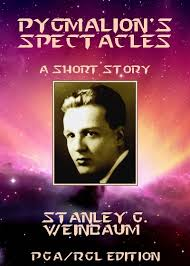
\includegraphics[scale=0.3]{pygmalion.jpeg}
\captionof{figure}{Couverture du livre \it{Pygmalion spectacles}\tss{\cite{pygmalion}}}
\end{center}

Un ancêtre de la réalité virtuelle est le View Master, développé en 1940 qui est un dispositif ressemblant à des jumelles qui fonctionne avec des cartes que l'on place dans une fente et on peut observer l'image en 3D. Cet appareil a déjà la forme du casque de réalité virtuelle qu'on connaît aujourd'hui.

\begin{center}
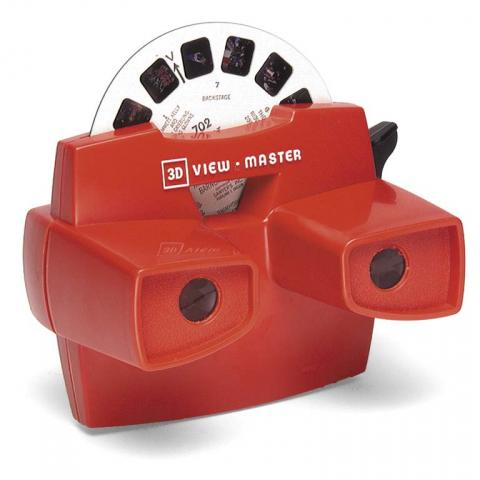
\includegraphics[scale=0.18]{viewmaster.jpg}
\captionof{figure}{Exemplaire du \it{View Master}\tss{\cite{viewmaster}}}
\end{center}


La première expériene véritable de réalité virtuelle a été permise en 1950 avec le Sensorama, un cinéma immersif créé par Morton Heilig. Grâce à son siège vibrant, il permet une totale immersion.
\begin{center}
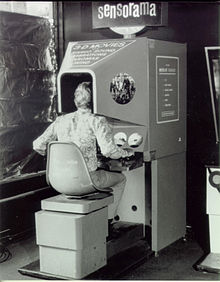
\includegraphics[scale=0.27]{sensorama.jpg}
\captionof{figure}{Modèle du Sensorama\tss{\cite{sensorama}}}
\end{center}



Cette ébauche de réalité virtuelle a servi d'ailleurs pour le développement d'un simulateur de vol pour l'armée de l'air en 1966. Le premier casque de réalité virtuelle a été créé en 1970, à l'Université d'Utah par Daniel Vickers. Il est formé de 2 écrans et permet d'observer l'image virtuelle en tournant la tête.
En 1982, les Data Gloves sont créés pour permettre une sensation de réalité virtuelle encore plus importante : ces gants se connectent à l'ordinateur et permettent d'effectuer des mouvements transmis à l'ordinateur.

\begin{center}
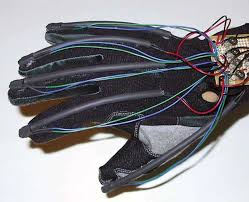
\includegraphics[scale=0.4]{data.jpeg}
\captionof{figure}{Photographie des Data Gloves de 1982\tss{\cite{data}}}
\end{center}

En 1989, la société VR qui est à l'origine des Data Gloves autorise Mattel, une entreprise de jeux de société, à modifier les Data Gloves pour pouvoir les intégrer à un jeu. Les Power Gloves sont alors commercialisés mais ils sont assez chers et donc peu populaires.
Avec l'arrivée d'Internet, la réalité virtuelle a été un peu délaissée et cette technologie est restée centrée sur les simulateurs de vol et la conception automobile, c'est-à-dire seulement dans des secteurs professionnels.

Vers 1990, la réalité virtuelle contamine enfin les jeux vidéos avec la création du casque SEGA VR, par la marque SEGA. Il est destiné à fonctionner avec la console MEGA VR. De plus, des gants exosquelettes permettent une plus grande interactivité entre la personne et l'environnement virtuel. Mais tous ces équipements coûtent jusqu'à 73 000\$ et sont donc peu accessibles pour le grand public.
\begin{center}
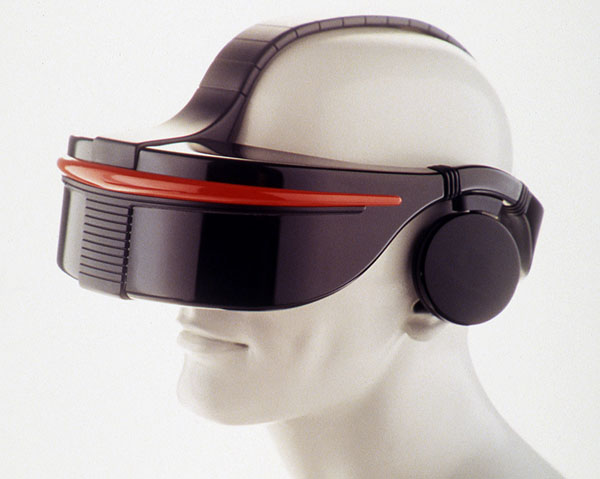
\includegraphics[scale=0.3]{sega.jpg}
\captionof{figure}{Le casque SEGA VR\tss{\cite{sega}}}
\end{center}

En 2007, Google créé Google Earth et Google Street View, deux logiciels qui permettent de visualiser les habitations et les rues grâce à une vision à 360\degres{}.\\
En 2014, Samsung créé son casque de réalité virtuelle, le Samsung Gear VR.\\
Le 5 avril 2016, le casque HTC Vive est commercialisé.\\
Le 28 mars 2016, Palmer Luckey créé l'Occulus Rift.
\begin{center}
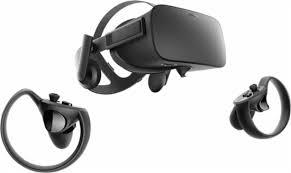
\includegraphics[scale=0.5]{occulus.jpeg}
\captionof{figure}{Le casque Occulus Rift\tss{\cite{occulus}}}
\end{center}
Mais le domaine de la réalité virtuelle est encore en plein développement !
Nous ne sommes donc qu'au début des innovations technologiques dans ce domaine.

\section[Catégories de casque]{Différentes catégories de casques de réalité virtuelle}

\paragraph{Les casques VR pour smartphones}

Certains casques doivent être utilisés avec un smartphone compatible. Ce casque est généralement passif. Il compte le plus souvent un système d'accroche, c'est à dire permettant la mise en place de deux lentilles qui font office de loupe. Cette méthode est la plus utilisée par les consommateurs car ces casques sont beaucoup moins coûteux que les casques autonomes. Il faut cependant un smartphone compatible et l'application pour l'utiliser. Le téléphone va donc s'occuper de tout le reste : les calculs, le rendu, l'affichage\ldots{}.

Un type très particulier de casque VR pour smartphone est le Google Cardboard. Créé par Google en 2014, ils sont fait principalement de carton (mais existent aussi en nylon et plastique) et permettent de tester la réalité virtuelle avec un budget très serré (prix minimal : 5\,\$). Ces petits boîtiers sont donc une bonne alternative pour tester la réalité virtuelle sans se ruiner. Nous en avons d'ailleurs acheté un pour pouvoir enrichir notre expérience.

\paragraph{Les casques autonomes}

Ils peuvent s'appuyer sur des capteurs de haute précision pour proposer une expérience d'immersion complète. De plus le spectateur peut aussi se déplacer librement au sein des environnements visionnés. Pour finir le casque autonome peut même retranscrire les mouvements du corps (s'accroupir, sauter\ldots{}). Les plus connus sont l'Occulus rift et l'HTC Vive. L'Occulus Rift, bien que très médiatisé, est assez peu utilisé par les professionnels car il est plutôt limité au niveau de ses capacités. L'HTC Vive, considéré comme le meilleur des casques, est très populaire puisqu'il satisfait aux contraintes des entreprises.

\section[Catégories de réalités]{Notion d'immersion, et différenciation des réalités}

\paragraph{L'immersion}

L'immersion désigne le fait d'être complètement plongé dans ou absorbé par quelque chose et ainsi pouvoir être plongé dans un autre monde. Ainsi, on peut être en immersion en lisant un livre passionnant comme on peut l'être avec un film effrayant. Il faut donc bien prendre en compte cette notion pour éviter l'amalgame entre réalité virtuelle et immersion.

\paragraph{Les nombreuses réalités différentes}

De nos jours, il existe de multiples catégories de réalité mais la majorité des gens pensent qu'il n'y a que la réalité virtuelle et associent donc des mauvaises définitions à ce terme. L'autre type de réalité qui se différencie le plus de la réalité virtuelle est la réalité augmentée.

Rappelons le, la réalité virtuelle repose sur l'impression de réel et surtout la possibilité d'interagir avec son environnement et son corps dans un environnement virtuel.

La réalité augmentée, quant à elle, repose sur l'ajout d'objets virtuels dans un environnement réel. Elle n'obstrue pas complètement, le plus souvent, le champ de vision du porteur du dispositif. Les caractéristiques de la réalité augmentée la rendent très attractive pour un secteur comme le tourisme. En effet, le fait de pouvoir ajouter des informations sur l'image vue par le porteur du dispositif peut par exemple servir à enrichir la visite d'un lieu touristique avec des informations complémentaires.

Le port de lunettes connectées fait partie de la réalité augmentée puisque l'utilisateur voit la réalité au travers de ses verres sur lesquels sont aussi projetés des objets numériques. Le champ de vision est tout de même plus limité que des lunettes classiques car il faut un espace assez grand pour permettre de projeter les objets virtuels.

\begin{center}
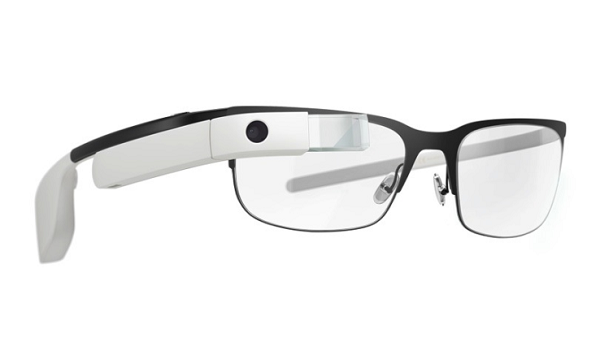
\includegraphics[scale=0.3]{glass.png}
\captionof{figure}{Photo du dispositif Google Glass\tss{\cite{formation}}}
\end{center}

On parle souvent de réalité virtuelle avec les vidéos à 360\degres{} proposées pour visiter les musées à distance avec un casque. Mais en réalité, elles ne se classent pas dans la réalité virtuelle : ce ne sont que des vidéos qui sont filmées et qui peuvent être diffusées ensuite mais qui ne permettent aucune interaction avec l'environnement virtuel et contraint l'utilisateur à être seulement spectateur, ce qui est contraire au principe de réalité virtuelle.

On peut voir que ces nouvelles technologies touchent de plus en plus les étudiants en informatique puisque lors de la porte ouverte de l'école Epitech, nous avons pu dialoguer avec un étudiant qui réalisait une application utilisant la réalité augmentée : cette dernière a pour but d'afficher des messages virtuels sur les batiments en ville, pour que les personnes utilisant l'application puissent les lire. Un autre étudiant a réalisé un logiciel de simulation de conduite utilisant la réalité virtuelle.

Nous nous restreindrons, dans ce dossier, à l'étude de la réalité virtuelle.

\chapter[l'\oe il et le cerveau]{Fonctionnement de l'\oe il et impact sur le cerveau}

L'\oe il est l'organe de la vision, sens qui permet à un être vivant de capter un signal lumineux, qui sera ensuite analysé par le cerveau.
L'\oe il a la capacité  de différencier près de huit millions de nuances de couleurs. Il participe activement à la perception de la réalité.

\begin{center}
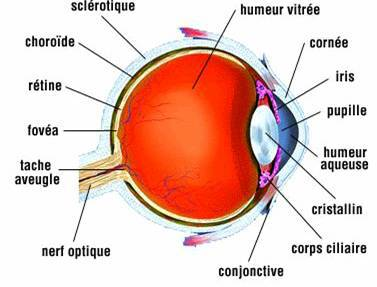
\includegraphics[scale=0.5]{oeil.jpg}
\captionof{figure}{Schéma détaillé de l'\oe il\tss{\cite{oeil}}}
\end{center}

L'\oe il est un globe entouré par la sclérotique, un tissu fibreux et opaque qui forme le blanc de l'\oe il et qui le protège des agressions extérieures tout en assurant le maintien de sa forme. La cornée quant à elle protège l'iris et le cristallin.

L'humeur vitrée est un liquide transparent gélatineux qui remplit l'intérieur de l'\oe il et en assure la forme.\\
L'humeur aqueuse, produite par le corps ciliaire, se trouve entre l'iris et la cornée et a pour rôle de nourrir la cornée et de protéger le cristallin. Ce liquide est renouvelé toutes les 4 heures.

L'iris est une membrane colorée qui se situe derrière la cornée et dont le diamètre peut varier à l'aide des muscles sphincters pour réguler la quantité de lumière qui entre dans l'\oe il.

Le cristallin est un organe particulier : il est dépourvu de tissu conjonctif, de cellules nerveuses et de capillaires sanguins. Ce dernier est composé de milliers de cellules allongées. Au centre du cristallin, les cellules sont parfaitement transparentes et la lumière peut donc passer.

Il est suspendu par des ligaments reliés aux muscles ciliaires. Lorsque ces derniers se contractent, cela provoque un glissement des cellules du cristallin pour que ce dernier prenne une forme plus bombée. Ce phénomène qui consiste à augmenter la vergence du cristallin pour voir nettement les objets proches s'appelle l'accommodation.

On peut ainsi assimiler le fonctionnement de l'\oe il à celui d'un appareil photo :
{\small}
\begin{center}
\begin{tabular}{|c|c|c|}
\hline Fonction de chaque composant & \'{E}léments de l'\oe il humain & \'{E}léments de l'appareil photo\\\hline
Régulation de la quantité de lumière& Iris & Diaphragme \\\hline
Formation de l'image & Cristallin & Lentille convergente \\\hline
Réception de l'image & Rétine & Capteur \\\hline
\end{tabular}
\captionof{figure}{Comparaison du fonctionnement de l'\oe il humain et de l'appareil photo\tss{\cite{photo}}}
\end{center}
{\small}

\begin{center}
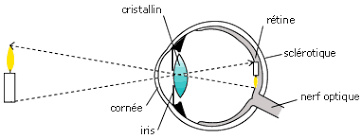
\includegraphics[scale=0.8]{schema_oeil.png}
\captionof{figure}{Schéma de la formation de l'image au niveau de l'\oe il\tss{\cite{formation}}}
\end{center}

\begin{center}
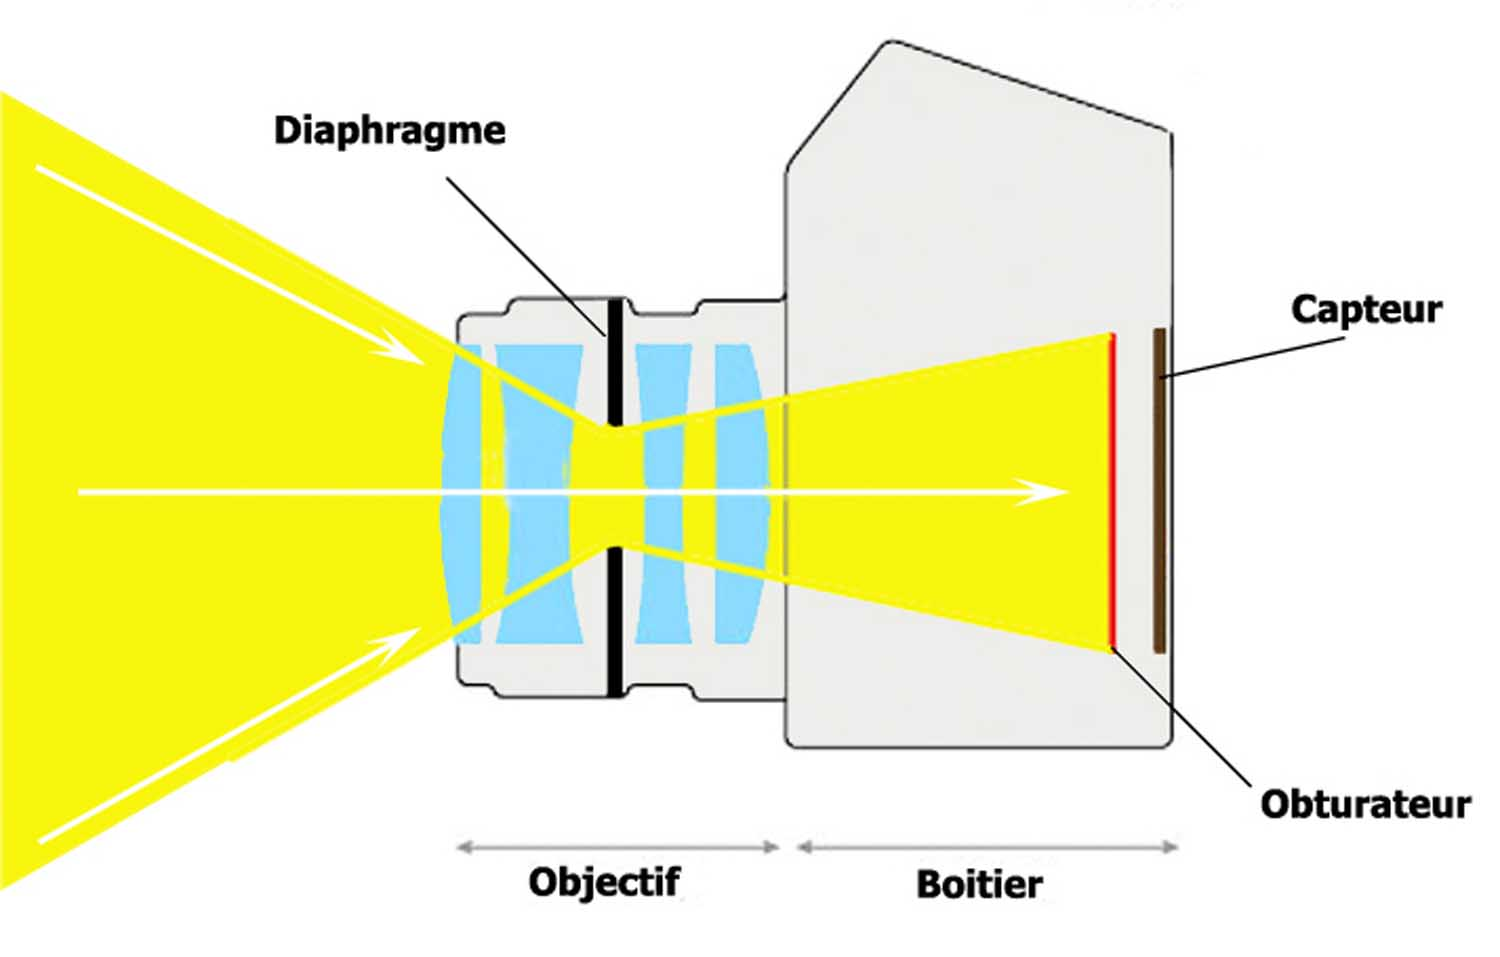
\includegraphics[scale=0.16]{appareil.jpg}
\captionof{figure}{Schéma de l'appareil photo simplifié \tss{\cite{photo}}}
\end{center}

On peut ainsi voir que l'\oe il et l'appareil photo, bien que très différents en apparence, se basent sur le même principe. L'image formée (voir schéma ci-dessus) se trouve sur la rétine, une fine membrane de 0,5\,mm d'épaisseur, transparente mais aussi incolore qui tapisse l'intérieur de l'\oe il. La région de la rétine sur laquelle l'image se forme se nomme la fovéa, située elle même sur la macula (région où sont concentrés les cônes). La fovéa mesure 1,5\,mm de diamètre.

\newpage{}

On peut constater que la rétine a une architecture complexe :
\begin{center}
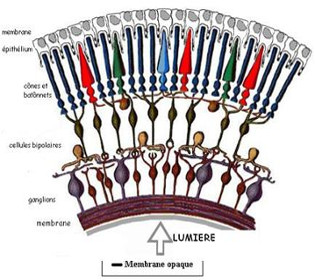
\includegraphics[scale=0.8]{retine.jpg}
\captionof{figure}{Composition de la rétine\tss{\cite{retine}}}
\end{center}

En effet on peut observer qu'elle possède de nombreuses couches. Tout d'abord, elle possède des photorécepteurs de deux types différents : les cônes et les bâtonnets. Les cônes sont responsables de notre perception des couleurs et il en existe 3 types différents : ceux sensibes à la couleur rouge, ceux sensibles à la couleur verte et ceux sensibles à la couleur bleue. Ils sont très concentrés au niveau de la fovéa. Les batonnets, eux, se trouvent sur la rétine périphérique : ils servent à capter la lumière de faible intensité. Ils sont 100 fois plus sensibles que les cônes.\\
Ensuite on peut voir deux couches de neurones : les neurones ganglionnaires et les neurones bipolaires. Ils ont pour rôle de transmettre les informations des photorécepteurs au nerf optique. Lorsque ces signaux électriques parviennent au nerf optique, ils sont acheminées vers le cerveau.\\

\begin{center}
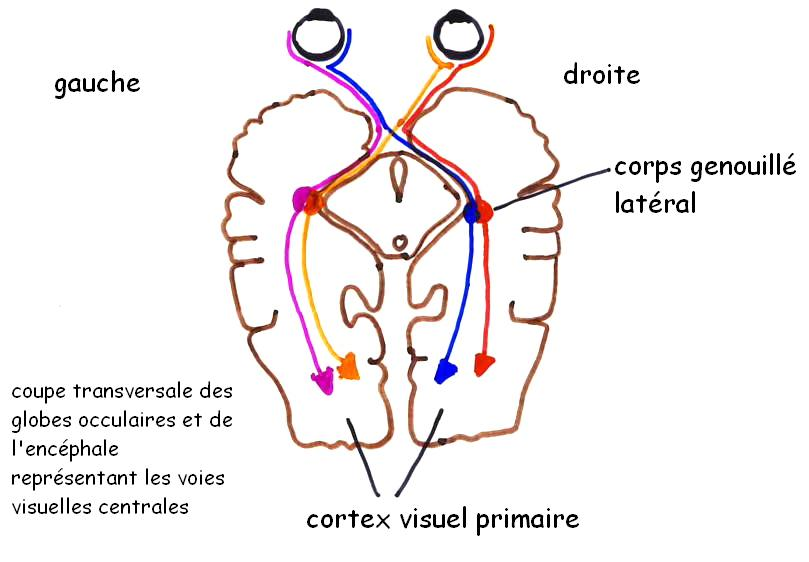
\includegraphics[scale=0.4]{cerveau.jpg}
\captionof{figure}{Schéma du cortex visuel et interaction entre le cerveau et l'\oe il\tss{\cite{cerveau}}}
\end{center}

Ces signaux électriques sont plus précisément au niveau de la partie arrière du cerveau : le cortex visuel. Pour cela, le corps genouillé latéral traite les informations de la rétine et les transmet au cortex visuel primaire. Ce dernier reçoit donc les signaux électriques des yeux et il chaque portion du champ de vision correspond à une région bien précise du cortex visuel primaire.

Cependant, le cortex visuel n'est pas la seule aire du cerveau à participer au processus de vision. Effectivement, on a pu constater qu'il y a au moins 5 aires cérébrales qui sont utiles à la création de l'image. Ces aires reçoivent des informations sur les formes, les mouvements\ldots{}

Le cerveau synthétise ensuite toutes ces informations, ce qui achève le processus de vision.

\chapter[Fontionnement]{Fonctionnement de la réalité virtuelle}

\section{Un exemple de casque autonome : L'HTC Vive}

L'HTC Vive est un casque de réalité virtuelle, né d'une collaboration entre HTC et Valve Corporation, qui est sorti le 5 avril 2016.
La version de test (le HTC Revive) avait des manettes filaires, alors que celles de la version finale sont sans fil.

\begin{center}
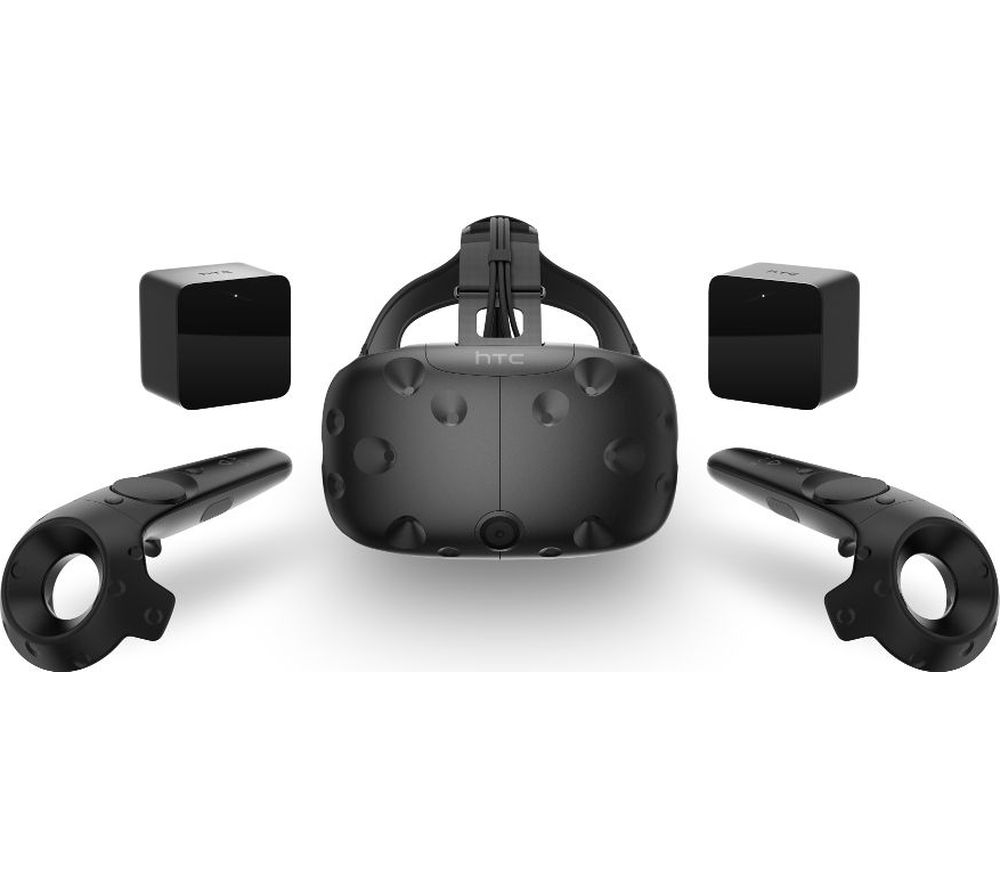
\includegraphics[scale=0.2]{htc.jpg}
\captionof{figure}{Le casque de réalité virtuelle HTC Vive\tss{\cite{htc}}}
\end{center}

\paragraph{Fiche produit :}
\begin{itemize}
\item Famille : Casque autonome
\item Environnement qui permet la bascule entre l'écran de l'ordinateur et celui du casque : Steam VR
\item Système d'exploitation nécessaire sur le PC pour utiliser le casque : Windows 7 ou plus récent
\item Résolution : 2160 $\times$ 1200 pixels (1200 $\times$ 1080 pixels pour chaque \oe{}il)
\item Taux de rafraichissement : 90\,Hz
\item Connectiques : HDMI, DisplayPort, USB, Jack
\item Fonctionnalités : L'HTC Vive est composé de capteurs comme le gyroscope, l'accéléromètre et les capteurs de position laser.
L'écart pupillaire peut se régler manuellement à l'aide d'une molette, située sur le coté droit du casque. La distance entre les yeux et les optiques se règle également à l'aide de deux autres molettes au niveau des attaches du casque.
Il comporte aussi une prise jack pour brancher des écouteurs ainsi qu'une prise USB pour des éventuelles extensions. Une caméra est intégrée sur la face avant, elle permet de voir l'environnement extérieur sans enlever le casque. Un micro permet quant à lui de parler dans les jeux multi-joueurs, ou de répondre à des appels téléphoniques via une connexion Bluetooth avec un téléphone portable.
\item Prix : 700\euro{} pour la version grand public et 1300\euro{} pour la version professionnelle.
\end{itemize}

\section[Fontionnement de l'HTC Vive]{Fonctionnement du casque autonome}

Que ce soit l'Occulus Rift, l'HTC Vive ou l'OS VR, ces casques se basent tous sur le même principe comme le montre le schéma ci-dessous.
\begin{center}
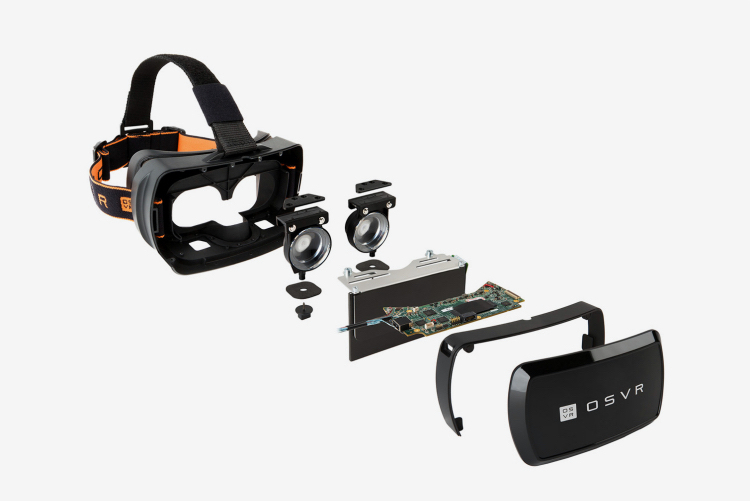
\includegraphics[scale=0.3]{eclate.jpg}
\captionof{figure}{Schéma éclaté d'un casque de réalité virtuelle\tss{\cite{eclate}}}
\end{center}

Tout d'abord, on peut voir que la structure du casque est pensée pour que l'utilisateur soit en position confortable durant l'utilisation. Le maintien est assuré par les nombreuses sangles qui compensent la masse importante du dispositif.

L'élément le plus fondamental est l'écran. Il doit posséder une excellente résolution car l'\oe{}il est situé très proche de ce dernier. Il est légèrement plus grand qu'un écran de smartphone, et comporte deux images, une pour chaque \oe{}il. Le casque fonctionne par stéréoscopie, technique grâce à laquelle le cerveau peut percevoir un relief. Ces images stéréoscopiques sont créées par deux lentilles situées en face de chaque \oe{}il. Enfin, on constate que les deux images sont légèrement décalées.

\begin{center}
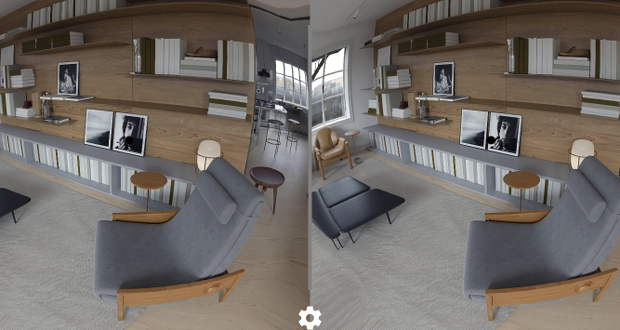
\includegraphics[scale=0.5]{ecran.jpg}
\captionof{figure}{Photographie représentant l'écran du casque\tss{\cite{ecran}}}
\end{center}

Il est nécessaire pour apprécier les distances, la profondeur, et le relief, que notre cerveau reçoivent des signaux électriques de nos deux yeux. C'est le même procédé qui est utilisé pour les manettes de la réalité virtuelle : elles comprennent 2 ou 3 caméras assurant une très grande précision.
Le champ de vision offert par le casque doit aussi être semblable à celui de l'\oe{}il en temps normal.

Pour permettre une meilleure immersion, des écouteurs sont intégrés au casque.
Des LEDs infrarouges, situées sur les lunettes et le bandeau arrière, permettent de détecter les mouvements de l'utilisateur. Une mini-caméra, placée à coté de l'utilisateur, localise le casque dans une zone de 9\,m\tss{2}.

Le logiciel Reality Adjacent Tracker assure le suivi des mouvements de la tête. Il combine trois technologies : l'accéléromètre pour mesurer les déplacements latéraux, le gyromètre qui est utilisé pour les mouvements de rotation et le magnétomètre qui agit comme une boussole.

Enfin, le délai entre le mouvement réel et sa retranscription à l'écran (latence) doit être très rapide pour vraiment donner l'impression de réel : pour l'Occulus rift, ce temps est de 25 millisecondes et pour l'HTC Vive, il est de 10 millisecondes environ. Ce temps de latence, s'il est trop long, peut provoquer la nausée.

\section[\'{E}tude statistique]{\'{E}tude de la popularité de la réalité virtuelle}

Pour connaître la popularité de la réalité virtuelle, nous avons décidé de réaliser un sondage au niveau du lycée sur ce sujet. Nous avons posé 8 questions aux 1545 élèves du lycée, à l'aide du site internet Survio. Nous avons 547 réponses, ce qui représente plus d'un tiers des élèves. Nous n'avons pu exploiter que 203 réponses sur les 547, puisque le lycée a refusé de financer l'accès complet aux résultats, payant sur ce site.

\begin{center}
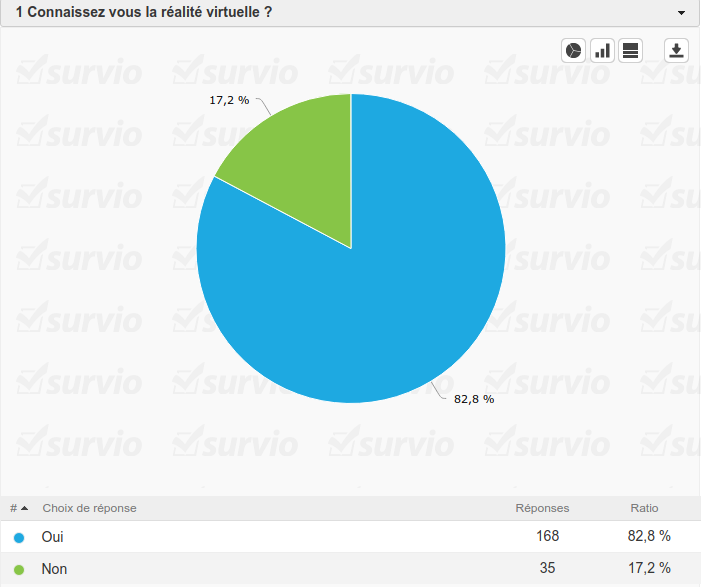
\includegraphics[scale=0.5]{1.png}
\captionof{figure}{Diagramme circulaire pour la question n\degres{}1\tss{\cite{etude}}}

La majorité des élèves a déjà entendu parlé de la réalité virtuelle.
\end{center}

\begin{center}
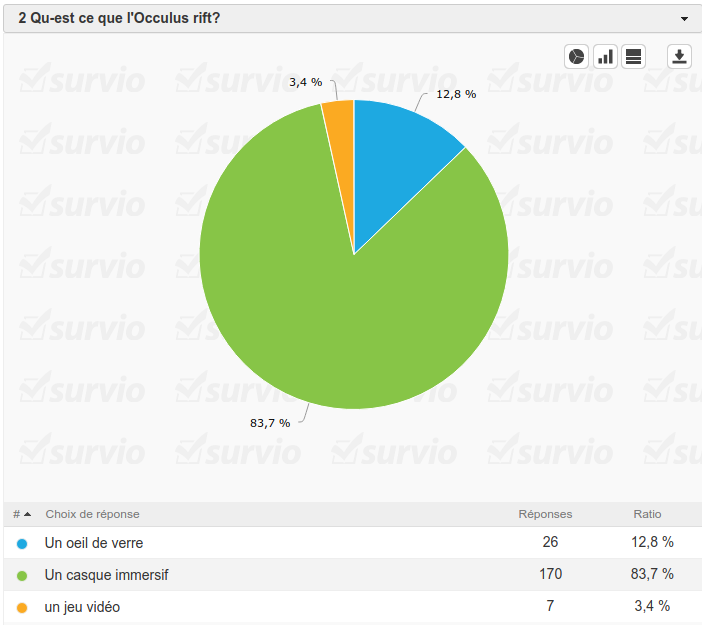
\includegraphics[scale=0.5]{2.png}

La plupart des jeunes savent ce qu'est un Occulus Rift mais 16,2\,\% de ces derniers se sont quand même trompés.
\end{center}

\begin{center}
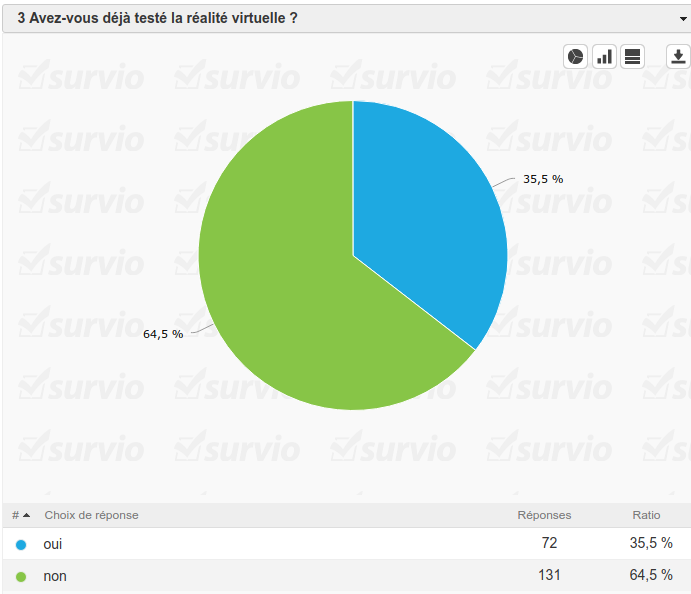
\includegraphics[scale=0.5]{3.png}

La majorité des jeunes n'a donc pas encore eu l'occasion de tester la réalité virtuelle.
\end{center}

\begin{center}
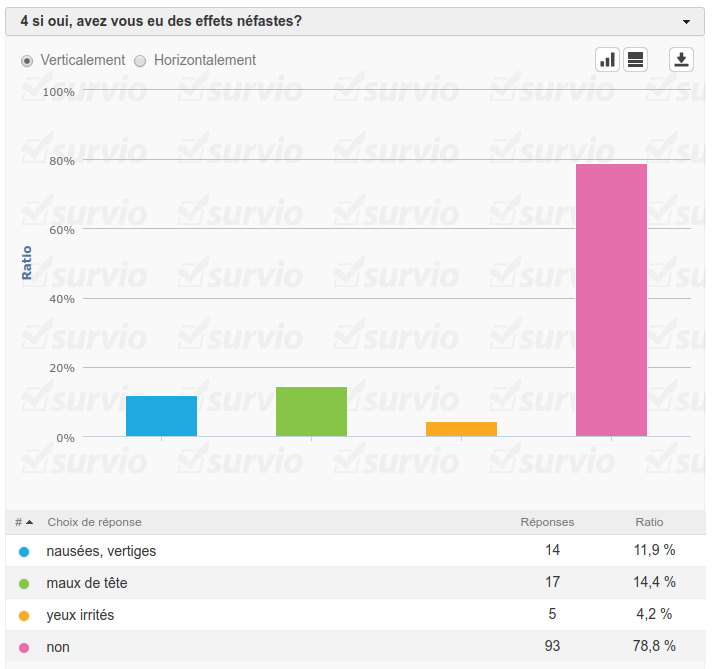
\includegraphics[scale=0.5]{4.png}

Seul environ 20\,\% des élèves a ressenti des effets néfastes lors de l'utilisation d'un casque VR.
\end{center}

\begin{center}
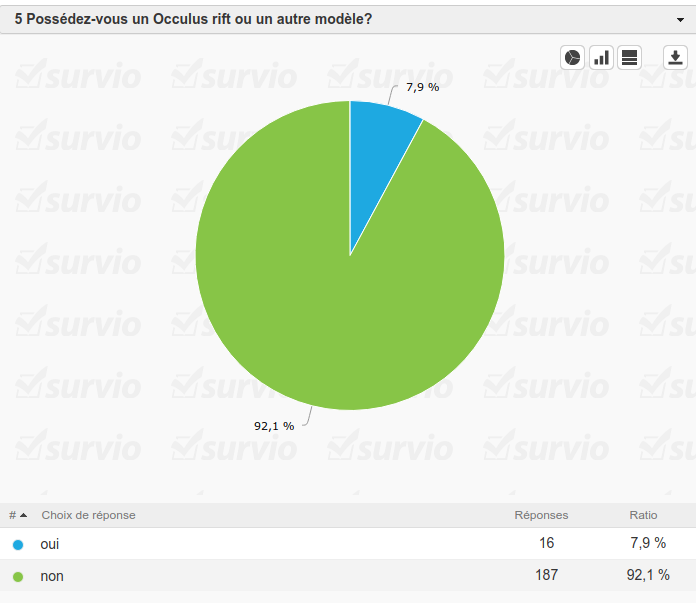
\includegraphics[scale=0.5]{5.png}

Moins d'un élève sur 10 en possède un.
\end{center}

\begin{center}
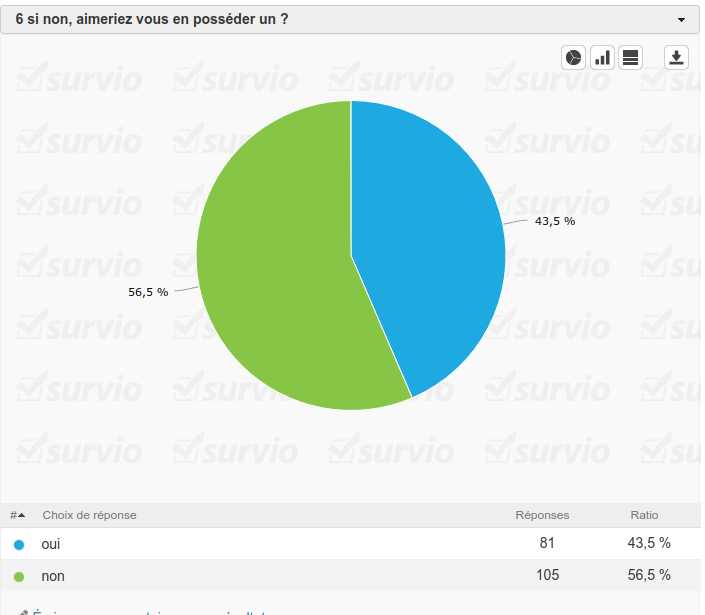
\includegraphics[scale=0.5]{6.png}

Moins de la moitié des jeunes interrogés désirent acquérir un casque VR.
\end{center}

\begin{center}
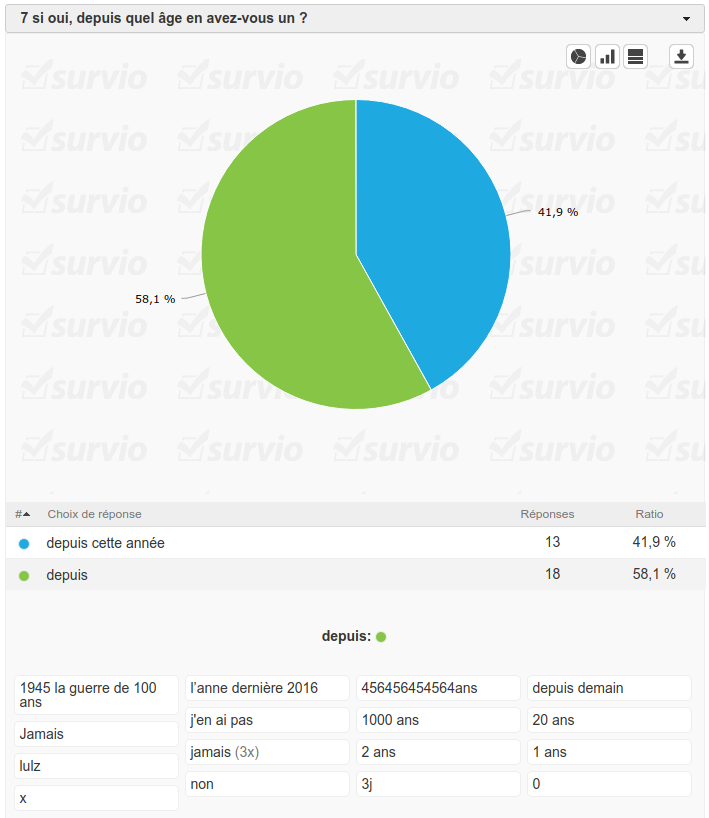
\includegraphics[scale=0.4]{7.png}

Compte-tenu du caractère plutôt imprécis de notre question, les résultats se sont révelés inexploitables.
\end{center}

\begin{center}
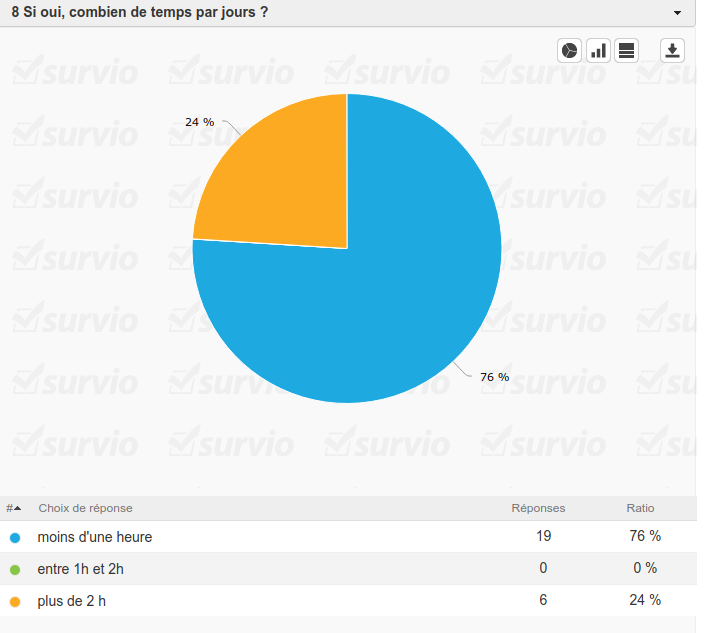
\includegraphics[scale=0.5]{8.png}

Nous pouvons constater ici que la majorité des jeunes est raisonnable dans l'utilisation de l'Occulus Rift.
\end{center}

\newpage

\section[\'{E}xpérience et sensations]{Expérience avec la VR et sensations éprouvées}

Nous voulions, pour enrichir notre TPE et avoir notre propre expérience, tester la réalité virtuelle et avoir l'avis d'un professionnel sur le sujet. Après de nombreuses recherches sur les différentes entreprises utilisant la réalité virtuelle, nous avons choisi de contacter l'école d'informatique  Epitech à Nancy et l'entreprise Human Games.

Epitech est un réseau d'écoles d'informatique dont une est située à Nancy. Nous y sommes allés lors des portes ouvertes et nous avons pu visiter l'établissement et poser quelques questions sur la réalité virtuelle. Nous avons également pu recueillir des témoignages d'étudiants qui avaient réalisé des logiciels utilisant ces nouvelles technologies. Grâce à ce témoignage, nous avons pu enrichir notre dossier.

L'entreprise Human Games, que nous avons contacté ensuite, nous a permis de tester un casque de réalité virtuelle : l'HTC Vive.

\begin{center}
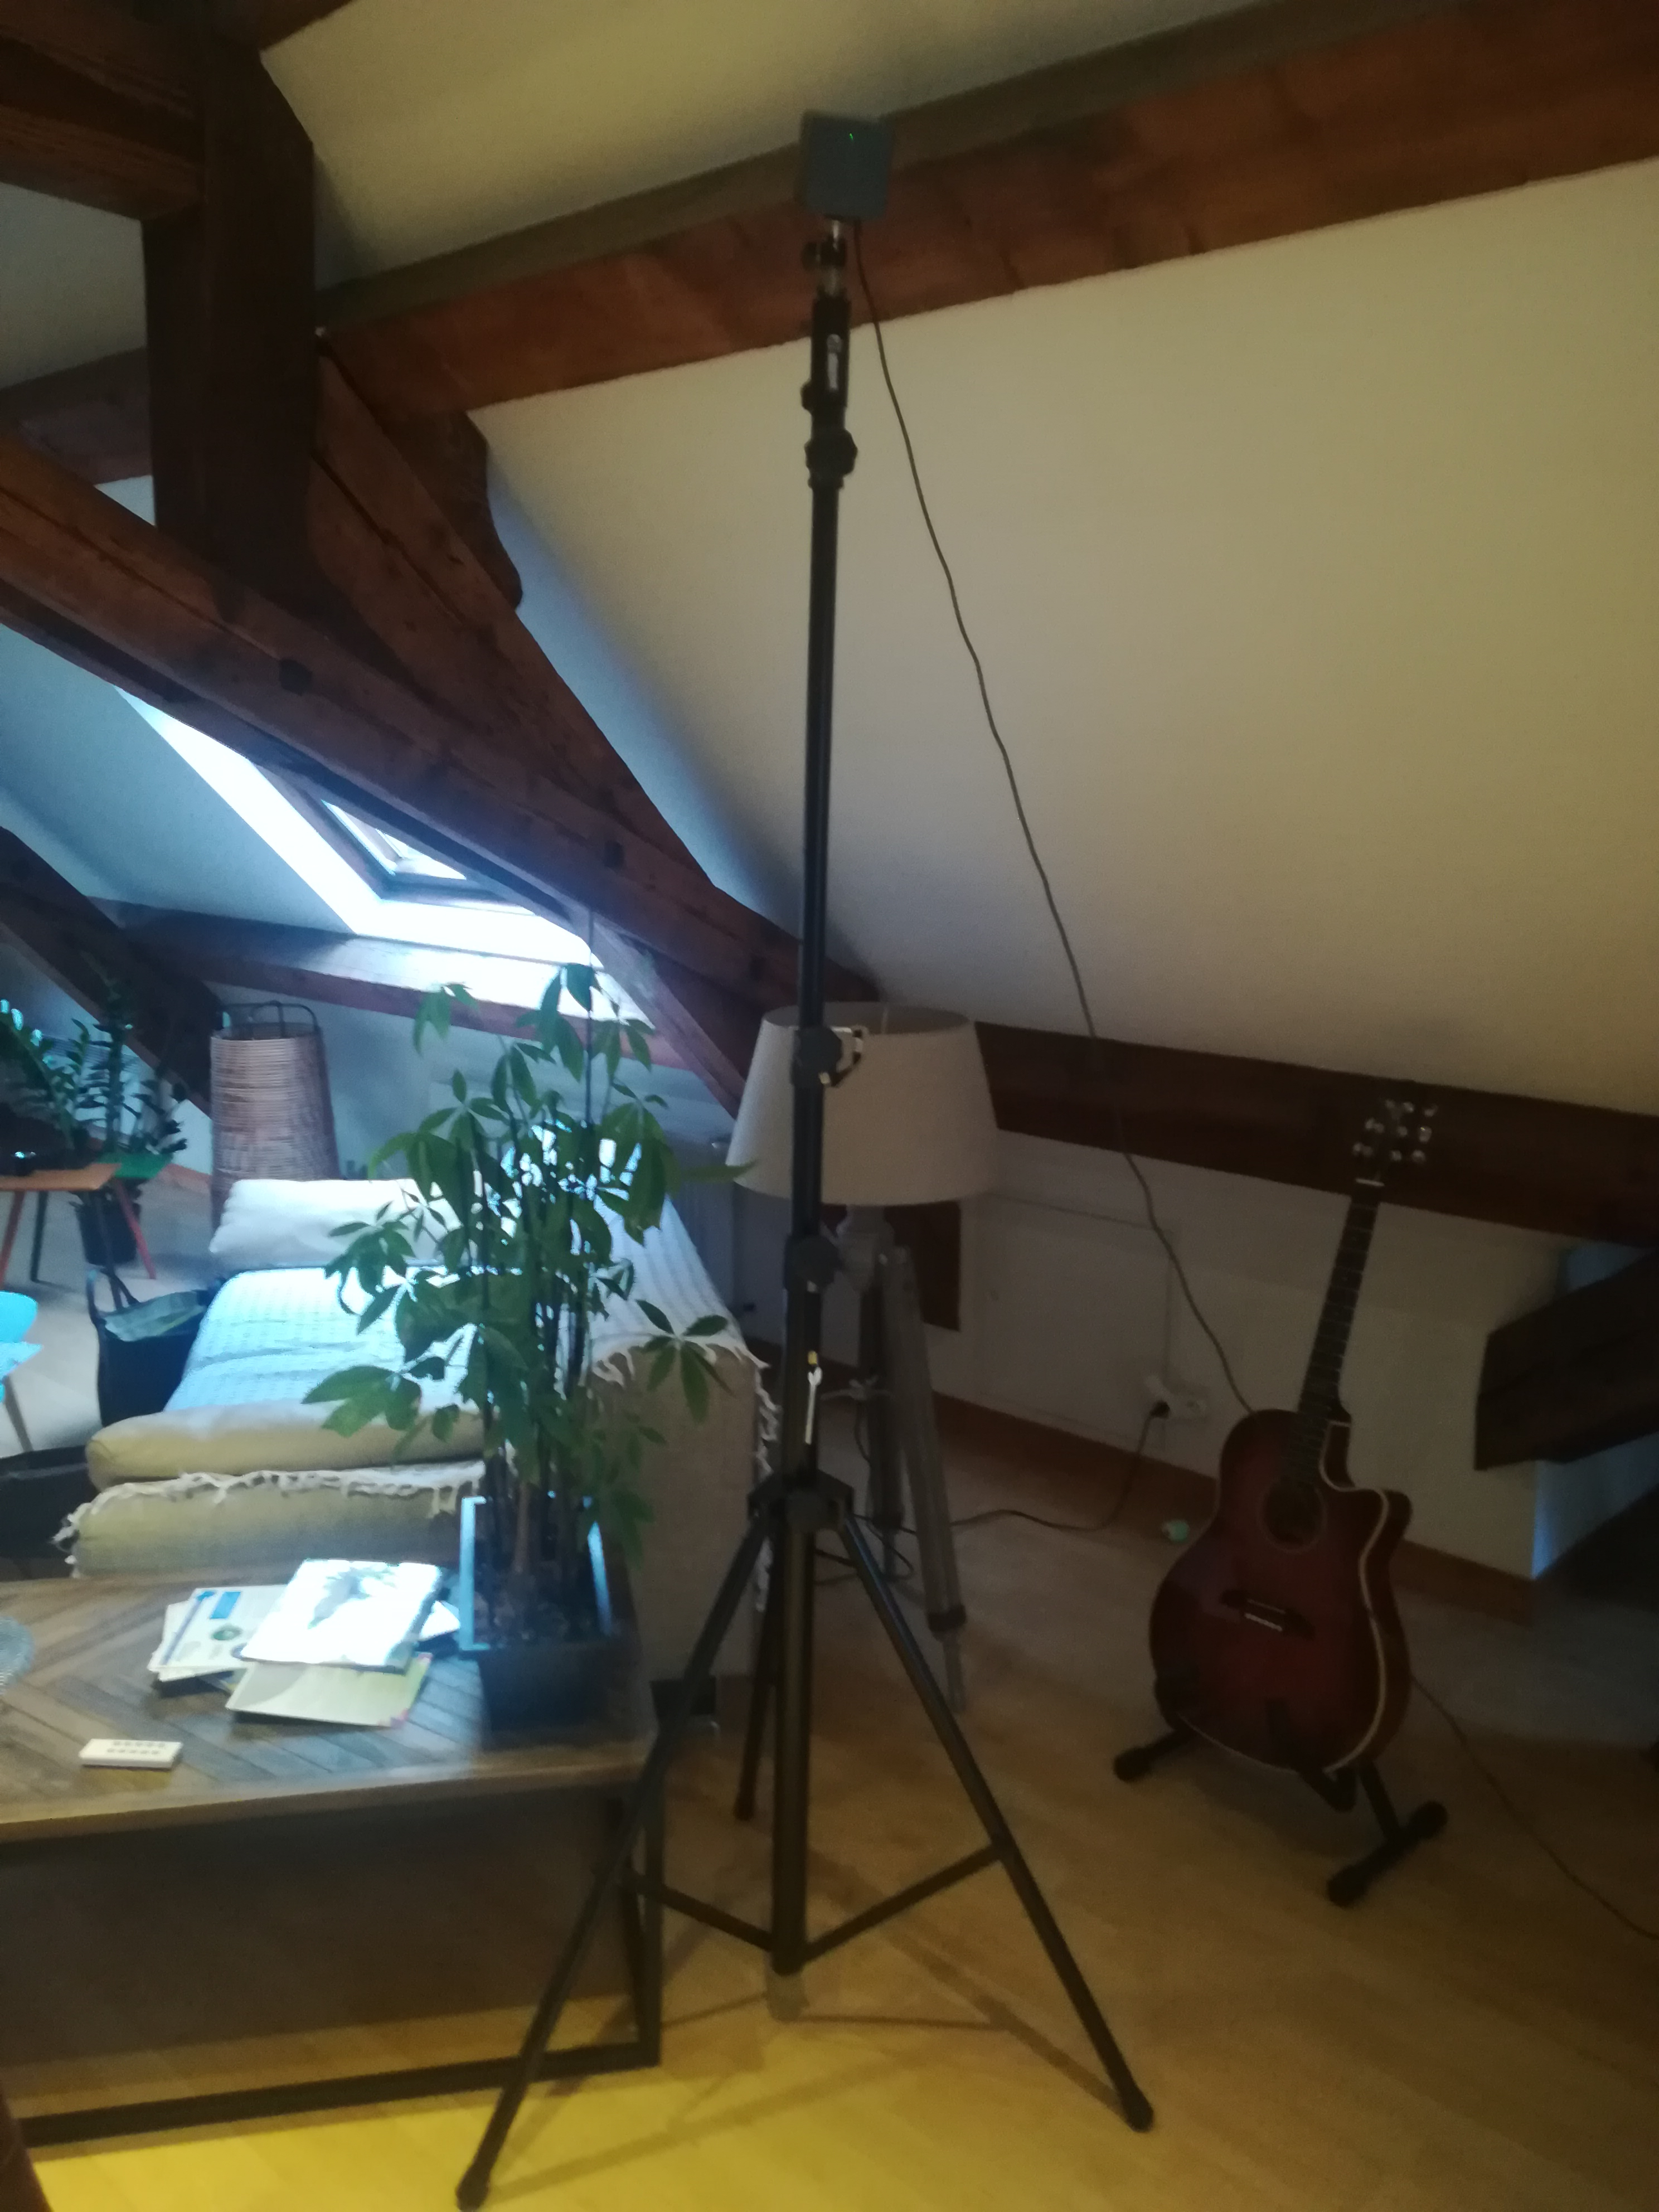
\includegraphics[scale=0.04 ]{capteur.jpg}
\captionof{figure}{Photographie d'un capteur nécessaire pour le fonctionnement du casque}
\end{center}


\begin{center}
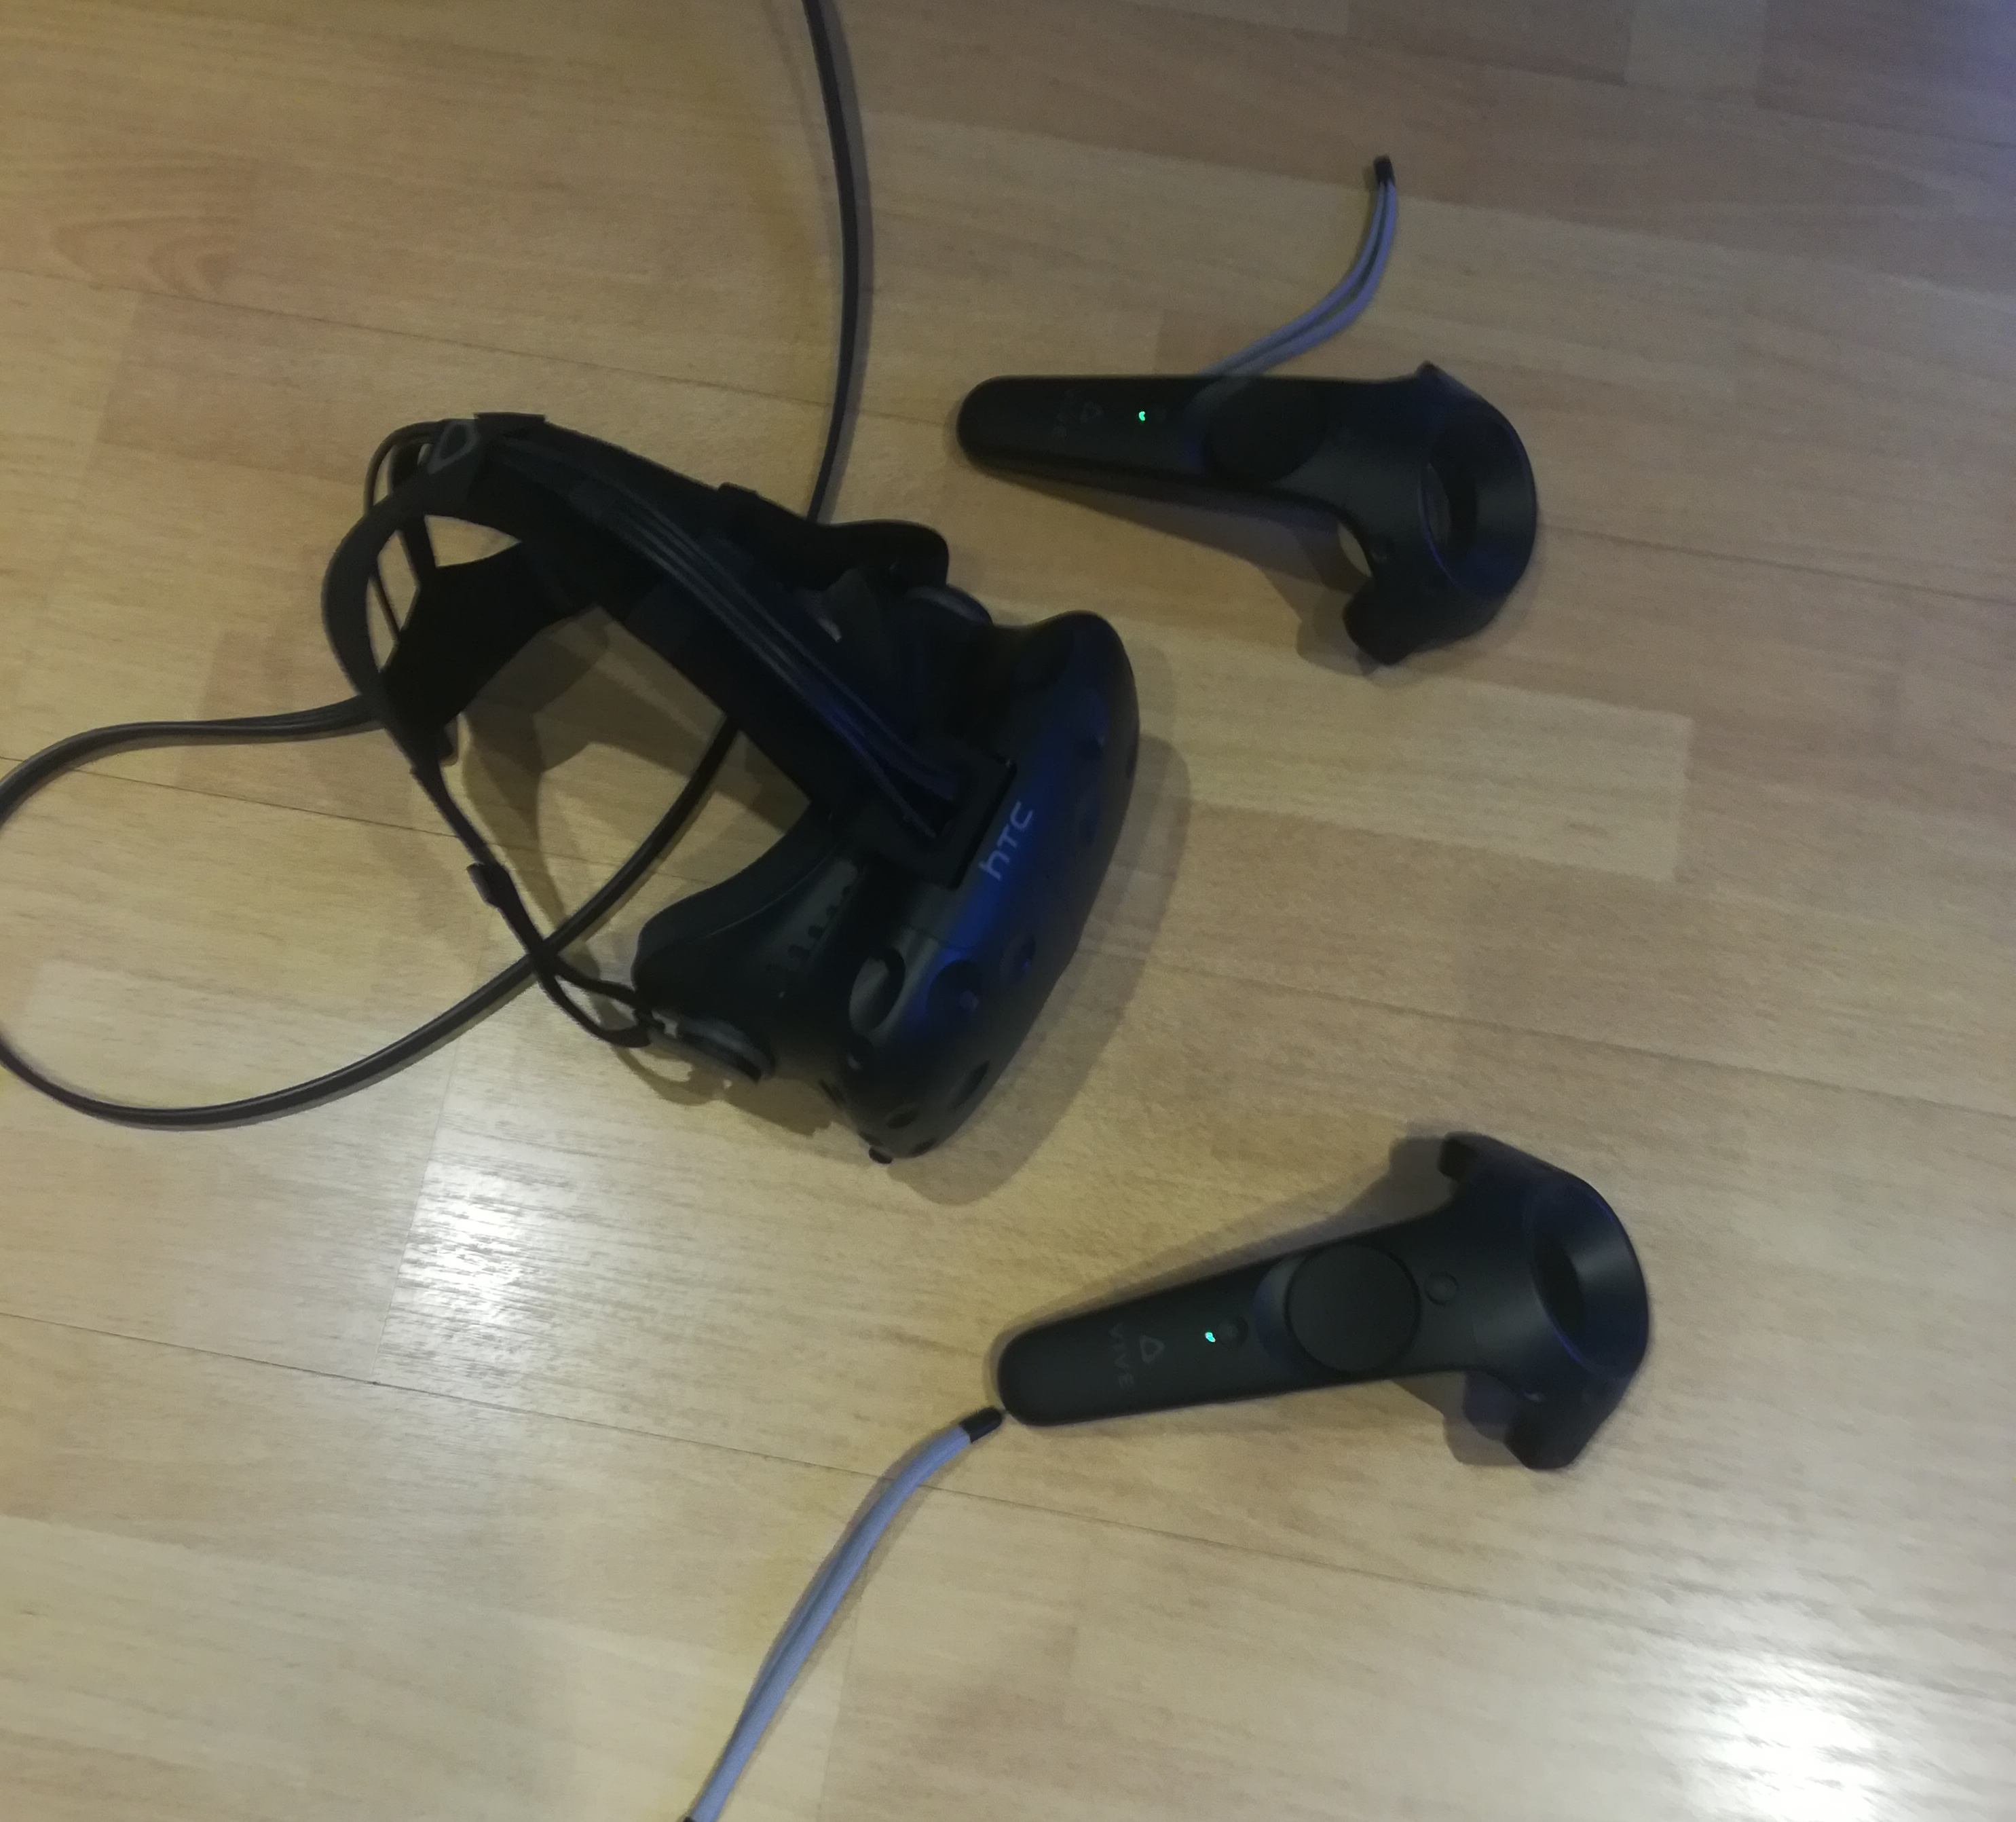
\includegraphics[scale=0.05]{casque.jpg}
\captionof{figure}{Photographie de l'HTC Vive}
\end{center}

\newpage{}

\begin{center}
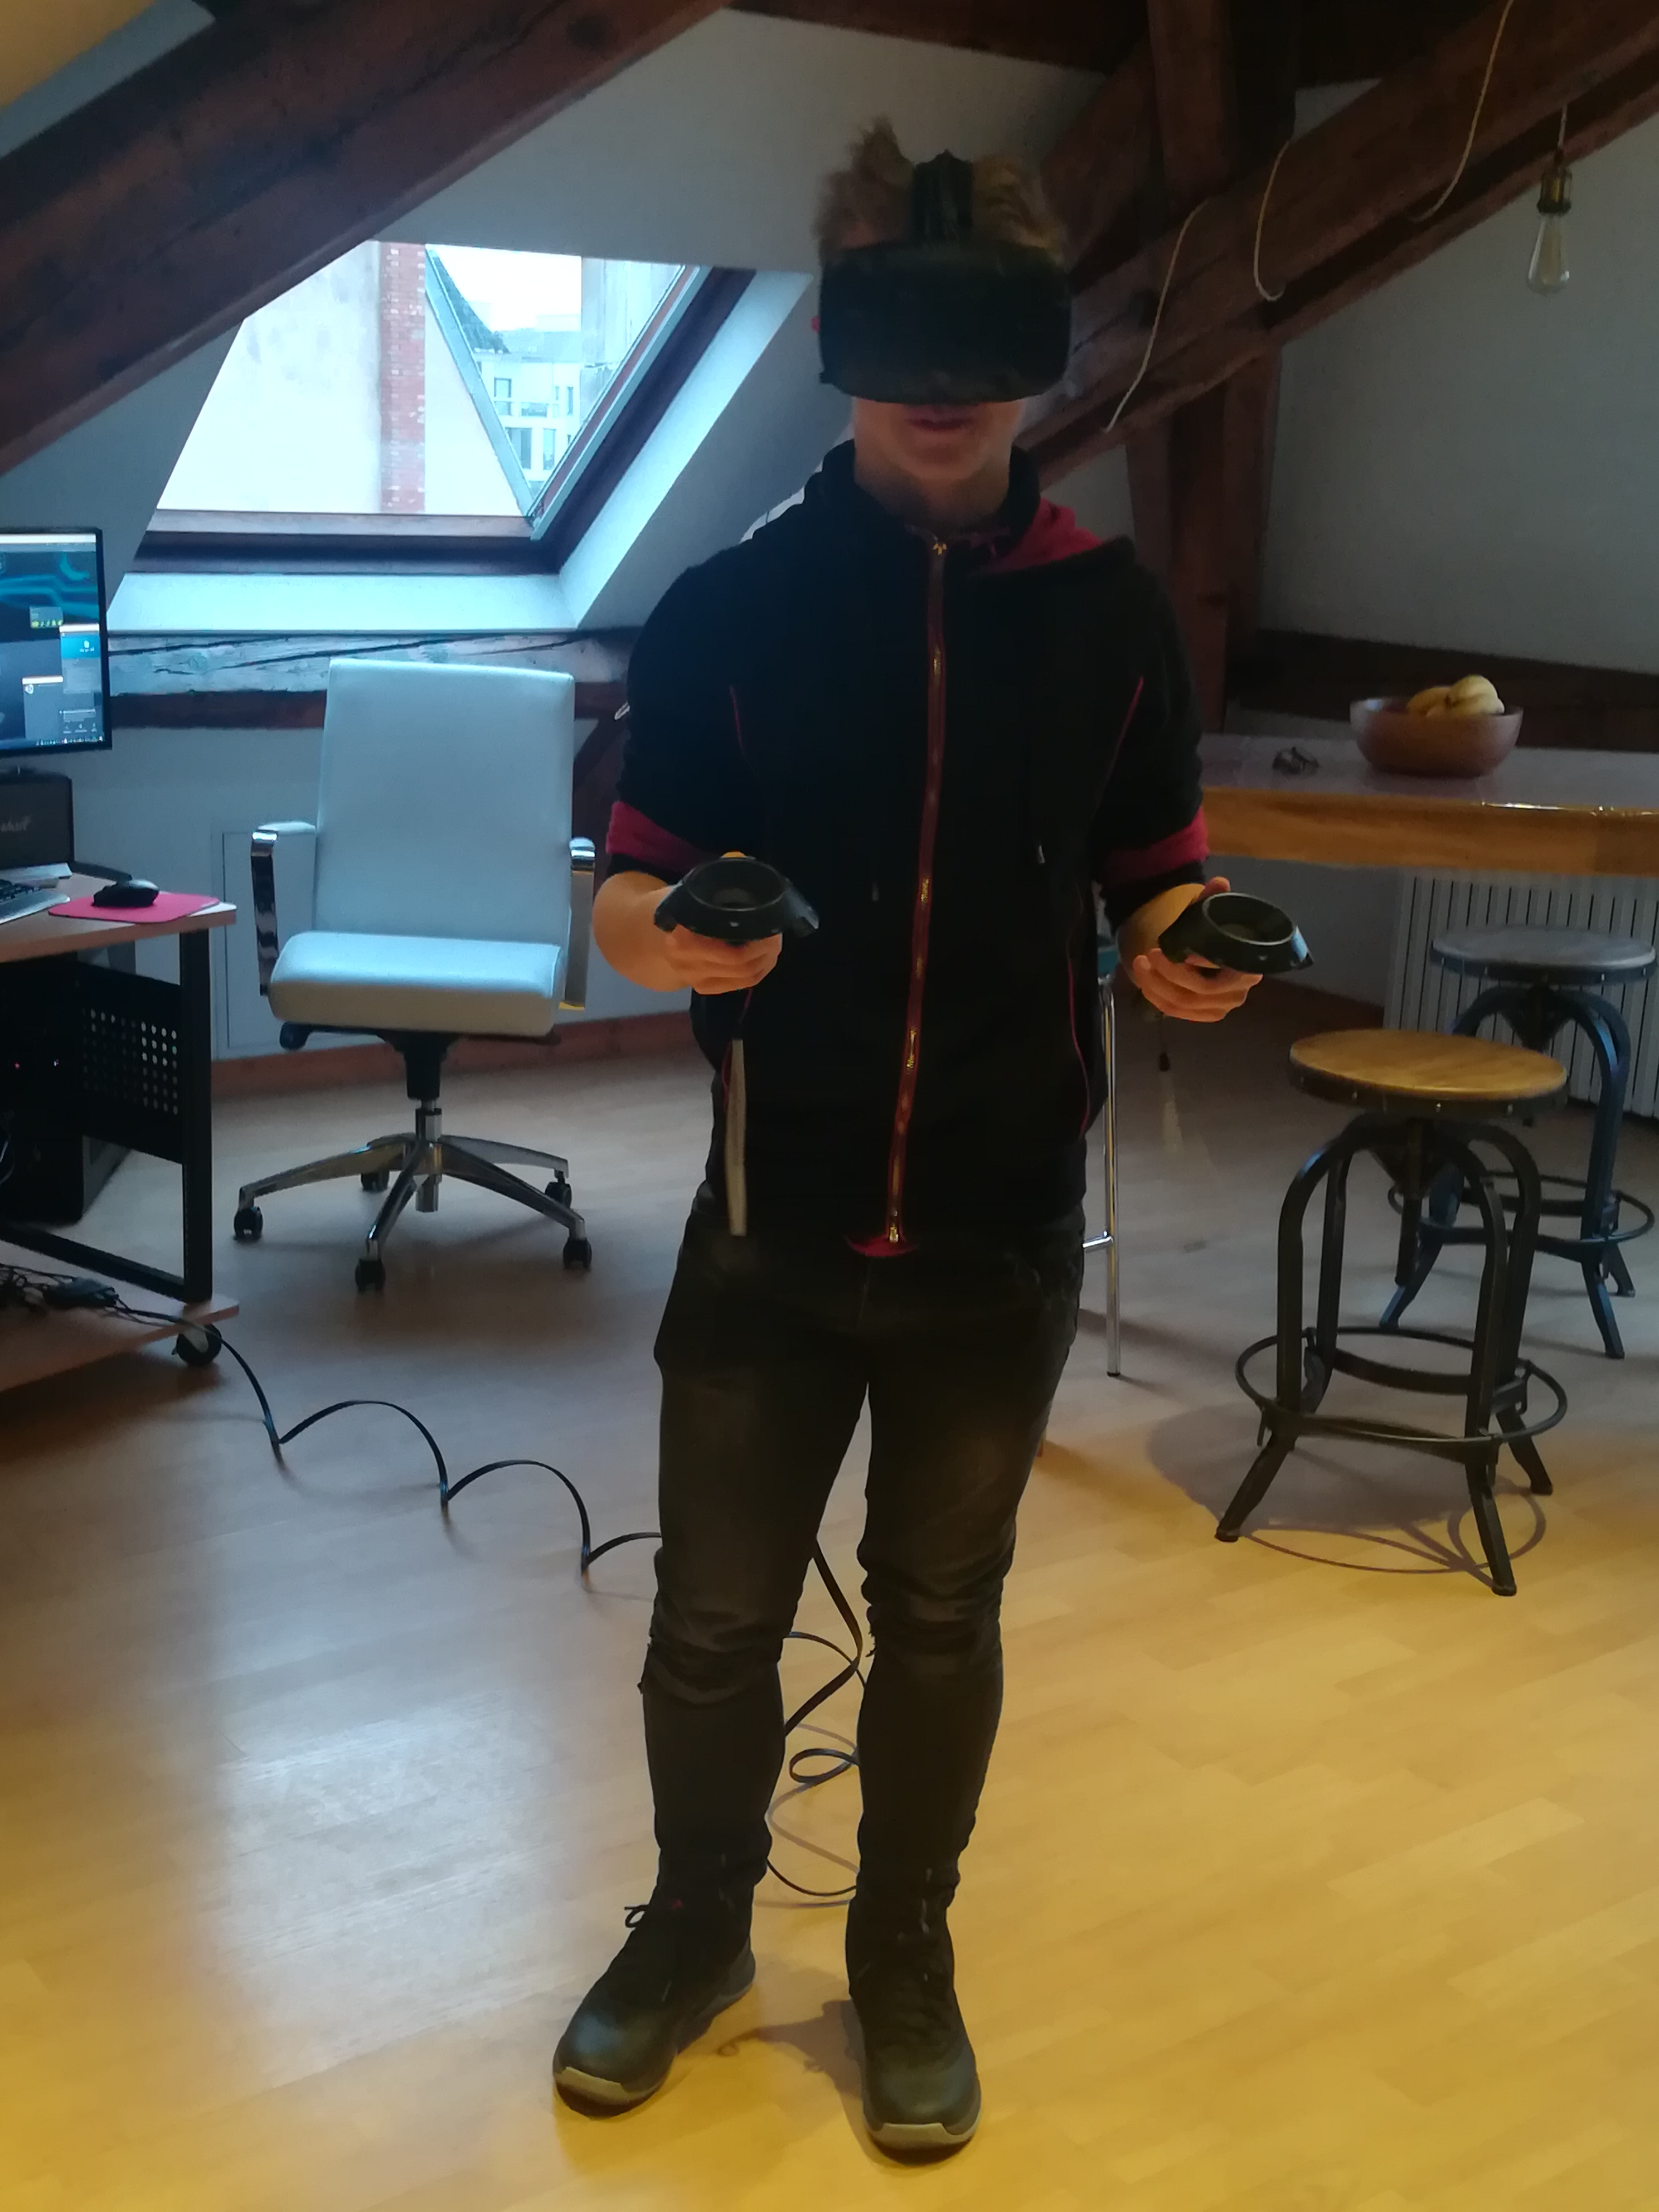
\includegraphics[scale=0.04]{nicolas.jpg}
\captionof{figure}{Nicolas prêt à utiliser le casque et les manettes}
\end{center}

Nous avons pu évoluer dans un environnement virtuel dans lequel de nombreuses activités nous étaient proposées : saisir un objet, mixer des sons, ou encore éclater des ballons. Ensuite, nous avons pu participer à une simulation sur le thème du gaspillage de l'eau. On pouvait évoluer dans une maison et prendre une douche, faire la vaiselle\ldots{} Nous avons également pu évoluer dans un environnement reproduisant une ville, et dans laquelle il nous était possible de marcher et même - sans douleur - de nous faire renverser par une voiture ! Les sensations étaient au rendez-vous ! L'immersion était totale et nous avons vraiment apprécié ce moment.

Durant l'expérience, aucune personne du groupe n'a ressenti d'effets néfastes mais juste après avoir retiré le casque, nous avons eu de légers vertiges et nous étions complétement déboussolés. Dans l'ensemble, cette expérience aura été très enrichissante.

\part[Changements et dangers]{Nombreux changements apportés par la réalité virtuelle et dangers relatifs à cette technologie}

\chapter[Innovations]{Innovations et changements apportés par la réalité virtuelle}

\section{Fonction ludique}

Si beaucoup de jeux vidéos disponibles pour la réalité virtuelle sont des adaptations de jeux existants pensés à la base pour la 2D, comme Resident Evil, Skyrim ou encore Until Dawn, de nouveaux jeux apparaîssent, compatible nativement avec la VR, pour le plus grand plaisir des joueurs.

Cependant, jouer à des jeux en réalité virtuelle reste encore très coûteux puisqu'il est nécessaire de posséder un ordinateur puissant et une carte vidéo de très bonne qualité (configuration avoisinant les 1000\euro) ainsi qu'un casque de réalité virtuelle (550\euro au minimum), soit un total de plus de 1500\euro{}, alors que les jeux classiques sont accessibles avec une configuration dès 600\euro.

Cependant la sortie récente du casque PlayStation VR (400 \euro et fonctionnant avec la PlayStation 4) permettra peut-être de faire baisser le prix des autres casques et de booster le développement des jeux spécialement conçus pour la réalité virtuelle.

\vspace{0.5cm}

\noindent Configuration minimale requise pour utiliser la VR avec une carte vidéo NVidia :
\begin{itemize}
\item GPU : Carte graphique NVIDIA GeForce GTX 1060 ou plus
\item CPU : Processeur Intel Core i5-4590 ou plus
\item Mémoire système : 8 Go de RAM ou plus
\item Sortie vidéo : HDMI 1.3 (x 1)
\item Connectique : USB 3.0 (x 3)
\item Système d'exploitation : Windows 7 Service Pack 1 (64 bits) ou plus
\item Pilote : GeForce 359 ou plus
\end{itemize}


\section[Avantages]{Les progrès et les avantages apportés par cette technologie}

La réalité virtuelle est en plein développement et mène une véritable révolution dans notre société. Cette technologie se répand dans plusieurs domaines comme la médecine, le sport ou encore la science ; elle va améliorer notre quotidien dans les années à venir.
Voici quelques aperçus de cette nouvelle technologie :
\begin{itemize}
  \item vivre sur Mars : la NASA prévoit d'utiliser la réalité virtuelle afin de simuler et d'expérimenter la vie sur la planète rouge. Cette technologie (simulation) entraîne efficacement les astronautes à l'environnement qu'ils devront affronter lors de leur mission ;

  \item apprendre à opérer : les étudiants en médecine vont pouvoir réaliser une opération virtuelle et être ainsi être mieux préparés à une opération.

  \item calmer la douleur : quand on ouvre les plaies des grand brûlés lors des séances de nettoyage, on place les patients dans un environnement virtuel représentant des terres gelées. Cela permet de calmer leur douleur sans avoir recours à la morphine ou une autre substance ayant la même visée, en modifiant la sécrétion d'endorphine, liée à la sensation de douleur. Cette hormone est produite par le complexe hypothalamo-hypophysaire, dont voici la localisation est produite ci-dessous. C'est ce dernier qui est responsable de la production de beaucoup d'hormones nécessaires au bon fonctionnement du corps humain ;
\end{itemize}

\begin{center}
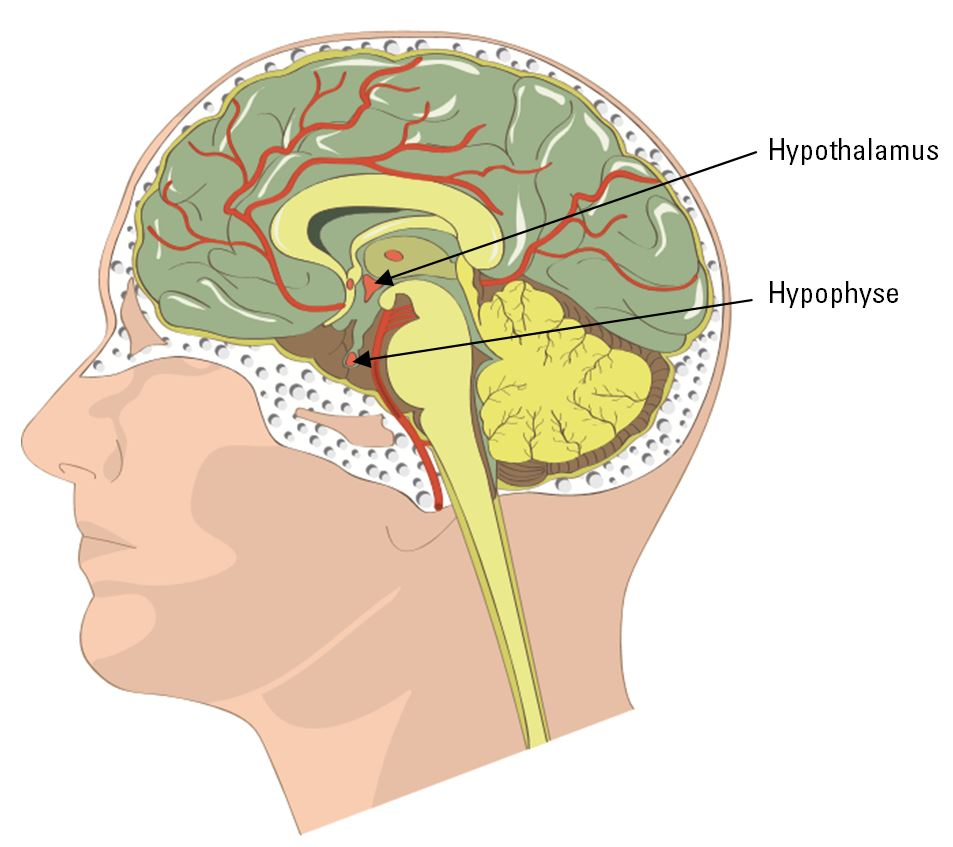
\includegraphics[scale=0.17]{cerv.jpg}
\captionof{figure}{Schéma du cerveau représentant le complexe hypothalamo-hypophysaire\tss{\cite{complexe}}}
\end{center}

\begin{itemize}
\item améliorer l'armée : la réalité virtuelle est utilisée dans l'armée pour améliorer l'entraînement des soldats dans des situations extrêmes sans leur faire courir aucun risque ;

\item faire du shopping : grâce à la réalité virtuelle, les clients auront la possibilité de se promener virtuellement dans les boutiques comme s'ils y étaient physiquement. Certains scientifiques cherchent même à développer un procédé qui permettrait de scanner nos corps afin d'essayer des vêtements à distance. Pour la marque Décathlon, la réalité virtuelle a permis aussi un gain de place dans les magasins et une meilleure promotion de leurs tentes Quechua. ``Aujourd'hui, la gamme étant composée de quatorze modèles allant de deux à huit places, il ne faudrait pas moins de 500\,m\tss{2} de surface pour pouvoir exposer tous les modèles et permettre à l'acheteur de trouver la tente idéale'', explique l'enseigne de sport dans un communiqué ;

\item simulateur de conduite : depuis quelques années certaines écoles de conduite proposent des cours de conduite en salle sur simulateurs. Ce sont de grosses machines qui sont très intéressantes pour des élèves en apprentissage de conduite. Ils peuvent travailler des notions spécifiques comme les démarrages ou arrêts ainsi que les changements de vitesse, permettant d'éviter sur la route les erreurs de débutant.\\
Cependant leur utilisation ne doit pas dépasser les 5 à 10\,h car il y a quand même une grosse différence entre des machines de réalité virtuelle de conduite et les sensations d'une vraie voiture dans un environnement réel ;

\begin{center}
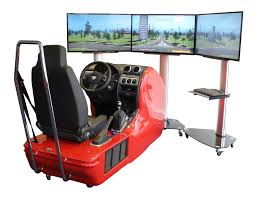
\includegraphics[scale=0.75]{onduite.jpg}
\captionof{figure}{Exemple de simulateur de conduite\tss{\cite{conduite}}}
\end{center}

\item simulateurs de vol : ils peuvent être utilisés pour le développement d'aéronefs, l'entrainement des équipages aux fonctions de bord (pilotage, navigation\ldots{}). C'est à l'heure actuelle l'usage le plus fréquent de la réalité virtuelle.

\begin{center}
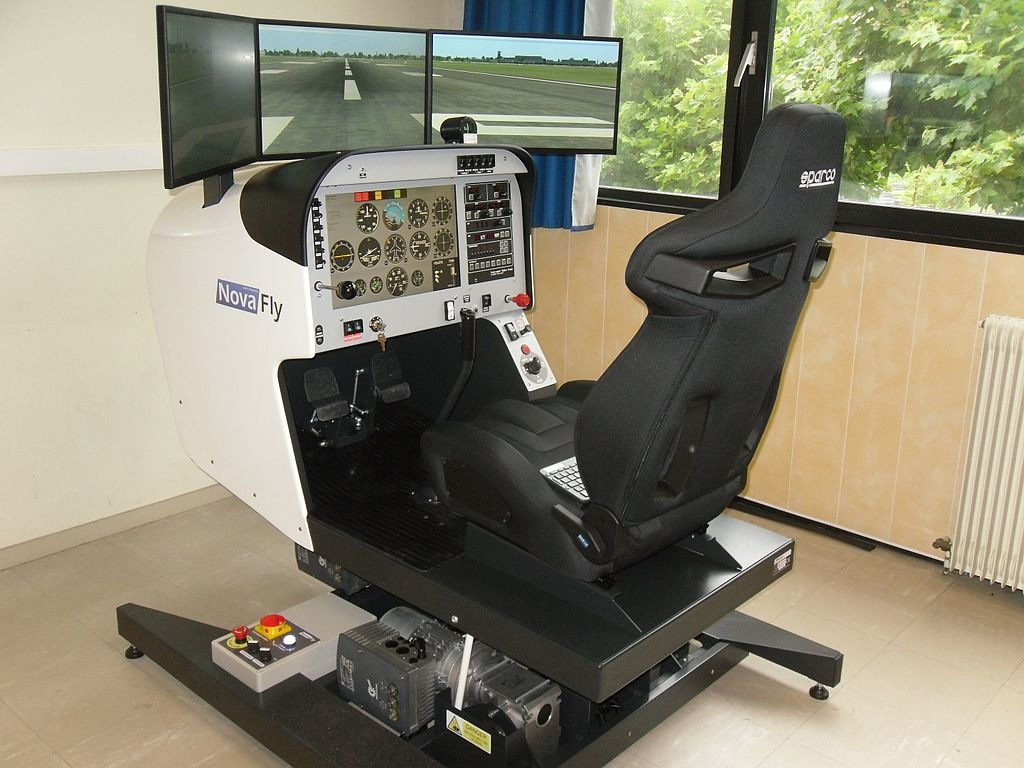
\includegraphics[scale=0.25]{conduite.jpg}
\captionof{figure}{Exemple d'un simulateur de vol\tss{\cite{vol}}}
\end{center}
\end{itemize}
\section[Peur et réalité virtuelle]{Combat et thérapie par la peur}

De nos jours, il existe de nombreux traitements pour les troubles ou les phobies grâce à l'utilisation de la réalité virtuelle.

D'après Eric Malbos, cyberthérapeute à l'hôpital de la Conception à Marseille, la réalité virtuelle est idéale pour le traitement des troubles anxieux, des phobies, des troubes obsessionnels et du stress post-traumatique.

La thérapie par la réalité virtuelle s'effectue sur le long terme. En effet le patient n'est pas plongé immédiatement dans un environnement virtuel. Tout d'abord, un diagnostic de la pathologie du patient est effectuée. Ensuite, des techniques de relaxation et de respiration lui sont enseignées pour lui apprendre à gérer son stress. Quand ce dernier est suffisament prêt, il est plongé -- toujours sous un contrôle médical strict -- dans un environnement virtuel dans lequel ce dernier affronte ses peurs.

\chapter[Dangers]{Les dangers pour la santé}

\section{Effets sur l'oeil}

A ce stade, la réalité virtuelle est une technologie assez nouvelle et il est donc difficile d'avoir du recul sur d'éventuels effets néfastes. Cependant, certains médecins émettent des hypothèses sur les éventuels effets néfastes occasionnés par la VR.

\subsection{Accomodation excessive} Les casques de réalité virtuelle reposent sur une très forte accomodation des yeux pour réussir à voir un unique objet alors que l'écran du casque en projette 2. Les médecins pensent donc qu'utiliser cette nouvelle technologie à très longue durée peut favoriser la perte de capacités d'accomodation et ainsi favoriser l'apparition de dommages au niveau de la vue.

\subsection{La lumière bleue, à ne pas négliger ?}

L'ANSES (Agence Nationale de Sécurité sanitaire, de l'alimentation, de l'Environnement et du travail) a récemment partagé ses inquiétudes concernant un autre risque encouru par les utilisateurs de la réalité virtuelle : celui d'abîmer irréversiblement la rétine, à cause de la lumière bleue.

Si l'on cherche à savoir pourquoi la lumière bleue semble incriminée, il faut définir ce qu'est une radiation lumineuse. \\ Une radiation lumineuse peut être décrite comme une onde ou comme une particule appelée photon. Cette particule se déplace à la vitesse de la lumière et ne possède ni masse, ni charge. L'énergie d'un photon est définie par la formule :
\begin{center}
 \Large{$\Delta E = \frac{h \times c}{\lambda}$}
\end{center}
 Avec $\Delta E$ le quantum d'énergie en $\mrm{J}$, $h$ la constante de Planck en $\mrm{J \cdot s^{-1}}$ et $c$ la célérité en $\mrm{m \cdot s^{-1}}$ ainsi que $\lambda$ en $\mrm{m}$. Or si on détermine le quantum d'énergie des longueurs d'ondes de $415$ à $450$ nanomètres (bleu), on obtient :
\[
\begin{array}{rcccl}
\Delta E_1 &=& \dfrac{6{,}63 \cdot 10^{-34} \times 3,0 \cdot 10^8}{415 \cdot 10^{-9}} &=& 4{,}79 \cdot 10^{-19}\u{J} \\

&&&&\\

\Delta E_2 &=& \dfrac{6{,}63 \cdot 10^{-34} \times 3,0 \cdot 10^8}{450 \cdot 10^{-9}} &=& 4{,}42 \cdot 10^{-19}\u{J}
\end{array}
\]

On obtient donc des valeurs comprises entre $ 4{,}42 \cdot 10^{-19}\u{J}$ et $4{,}79 \cdot 10^{-19}\u{J}$.

Or si on compare nos résultats au quantum d'énergie émis par un photon correspondant à une longueur d'onde proche de $700$ nanomètres (rouge), on obtient:
\begin{center}

\[
\Delta E_3 = \dfrac{6{,}63 \cdot 10^{-34} \times 3,0 \cdot 10^8}{700 \cdot 10^{-9}} = 2{,}84 \cdot 10^{-19}\u{J}
\]

\end{center}

On peut donc voir que le quantum d'énergie délivré par le photon responsable de la couleur rouge est une fois et demi inférieur à celui de la lumière bleue.

On comprend alors pourquoi la lumière bleue semble particulièrement dangereuse, car l'énergie qu'elle transporte, plus importante que pour les autres longueurs d'ondes, est directement absorbée par la rétine.

La réalité virtuelle ne semble donc pas vraiment faire bon ménage avec nos yeux !

\section{Effets sur l'équilibre}

En temps normal, le cerveau utilise trois sources de données pour informer l'organisme sur sa position et ses mouvements : l'oreille interne, les muscles et les yeux. Mais une fois le casque sur la tête, les yeux indiquent que l'on est en mouvement, mais l'oreille interne et les muscles disent que ce n'est pas le cas : cette incohérence des informations sensorielles peut provoquer des nausées. Le cerveau est donc perturbé et finit par envoyer des signaux d'alarmes, sous la forme de nausées. La sensation est similaire à celle ressentie par une personne malade en voiture.

L'oreille interne est la partie de notre corps qui assure l'équilibre ; ce rôle est plus précisément assuré par un organe sensoriel de l'oreille interne, l'appareil vestibulaire. Ce dernier détermine la position de la tête de l'individu dans l'espace et informe le cerveau de ses mouvements. Il permet donc de coordonner les mouvements de la tête et du reste du corps.

L'oreille interne est composée d'un réseau de cavités rigides creusées dans l'os temporal. Le vestibule, partie molle dans l'os temporal est composé de sacs, l'utricule et la saccule, mais aussi de trois canaux en demi-cercles, placés à la perpendiculaire les uns des autres, qui contiennent un liquide, l'endolymphe. En fonction des mouvements effectués par la tête, l'endolymphe s'y déplace dans un sens donné et cette information est captée par des récepteurs spécialisés, qui l'envoient au cervelet via le nerf vestibulaire.

Nous avons recueillit le témoignage de Franck Petriz, récemment diplomé de l'école Epitech Nancy, qui a réalisé un logiciel pour simulateur de conduite. Il a remarqué que pour atténuer l'effet de nausée avec les casques de VR, il fallait placer au niveau de l'écran un triangle noir statique, qui recrée l'absence d'image au niveau du nez.

\newpage{}

\begin{center}
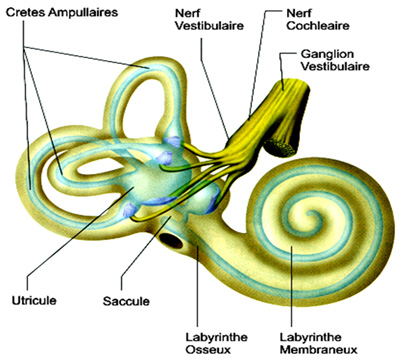
\includegraphics[scale=0.5]{oreille.jpg}
\captionof{figure}{Schéma de l'oreille interne\tss{\cite{oreille}}}
\end{center}

\section[Effets sur le cerveau]{Effets potentiels sur le cerveau}

Le professeur Mayank Mehta de l'université UCLA en Californie, étudie depuis 2009 les effets de la réalité virtuelle sur les neurones. Une expérience menée sur des rats placés dans un univers virtuel montre que 60\,\% des neurones de l'hippocampe, partie du cerveau dédiée à la mémoire et aux repères spatiaux, devenaient inactifs et que les 40\,\% restants fonctionnaient de façon chaotique. Le professeur a également noté une baisse sensible au niveau de l'activité électrique de tous les neurones. Même si l'étude a seulement été réalisée sur des rats, elle peut tout de même donner des informations à propos des effets sur l'homme. Le professeur et son équipe travaillent d'ailleurs actuellement sur une technologie qui leur permettra de comprendre ce qu'il se passe à l'intérieur d'un neurone chez un sujet placé dans un univers virtuel.

\appendix

\addcontentsline{toc}{part}{Annexes}

\chapter*{Conclusion}
\addcontentsline{toc}{section}{Conclusion}

Mais alors, que dire de la réalité virtuelle ? Est-ce un bienfait ou est-ce néfaste ?

Nous avons analysé les principales hypothèses sur les dangers de la réalité virtuelle mais nous nous sommes rendus compte qu'il était très difficile de mesurer à l'heure actuelle les dangers et risques pour l'organisme. En effet, les scientifiques n'ont pas un recul suffisant sur cette technologie pour tirer des conclusions. Cependant, on constate que cette technologie permet déjà de nombreux progrès dans des domaines variés.

Au final, il convient de profiter des bénéfices apportés par la VR tout en restant très prudent. Tout d'abord, il convient d'interdire la VR aux enfants de moins de 12 ans dont le système visuel et le cerveau ne sont pas complètement matures. Il est également important d'adopter une utilisation raisonnée de la réalité virtuelle, en faisant par exemple des pauses toutes les heures, comme le préconisent les fabriquants.

Toutefois, à la suite de cette étude, nous pensons qu'une utilisation trop importante des dispositifs de réalité virtuelle par des personnes plutôt instables psychologiquement peut mener à un isolement total, à des troubles psychologiques ainsi qu'une confusion complète entre la réalité et le virtuel.

\chapter*{Remerciements}
\addcontentsline{toc}{section}{Remerciements}

Nous voulons remercier de nombreuses personnes sans qui nous n'aurions pu réaliser ce travail.

Tout d'abord, nous remercions notre professeur référent, M. \sc{Julian}, qui nous a suivi et conseillé durant tout notre projet, ainsi que tous les autres profeseurs de TPE et de l'établissement qui ont pu nous apporter leur aide.

Nous remercions aussi tous les élèves de l'établissement Arthur \sc{Varoquaux} qui ont pris sur leur temps pour répondre à notre sondage et qui nous ont permis de récolter toutes ces données.

Nous voulons remercier tout spécialement l'entreprise Human Games qui nous a chaleureusement acueilli dans ses locaux et qui nous a permis d'expérimenter la réalité virtuelle et d'obtenir de précieux conseils pour ce projet. Sans eux, nous n'aurions pas pu mesurer réellement les enjeux de cette nouvelle technologie.

Enfin, nous remercions tous nos proches pour avoir pris de leur temps pour nous relire et nous conseiller sur ce rapport.

\addcontentsline{lof}{part}{Annexes}

\chapter*{Google Cardboard}
\addcontentsline{toc}{section}{Google Cardboard}

En vue de l'oral du TPE, qui aura pour but de présenter notre projet, nous nous sommes dit qu'il faudrait que le jury puisse tester la réalité virtuelle pour ainsi mieux comprendre nos propos. Pour cela, nous avons acheté un Google Cardboard (au prix de 6\,\euro) qui, accompagné d'un télephone compatible, va permettre de simuler un casque de réalité virtuelle.

\begin{center}
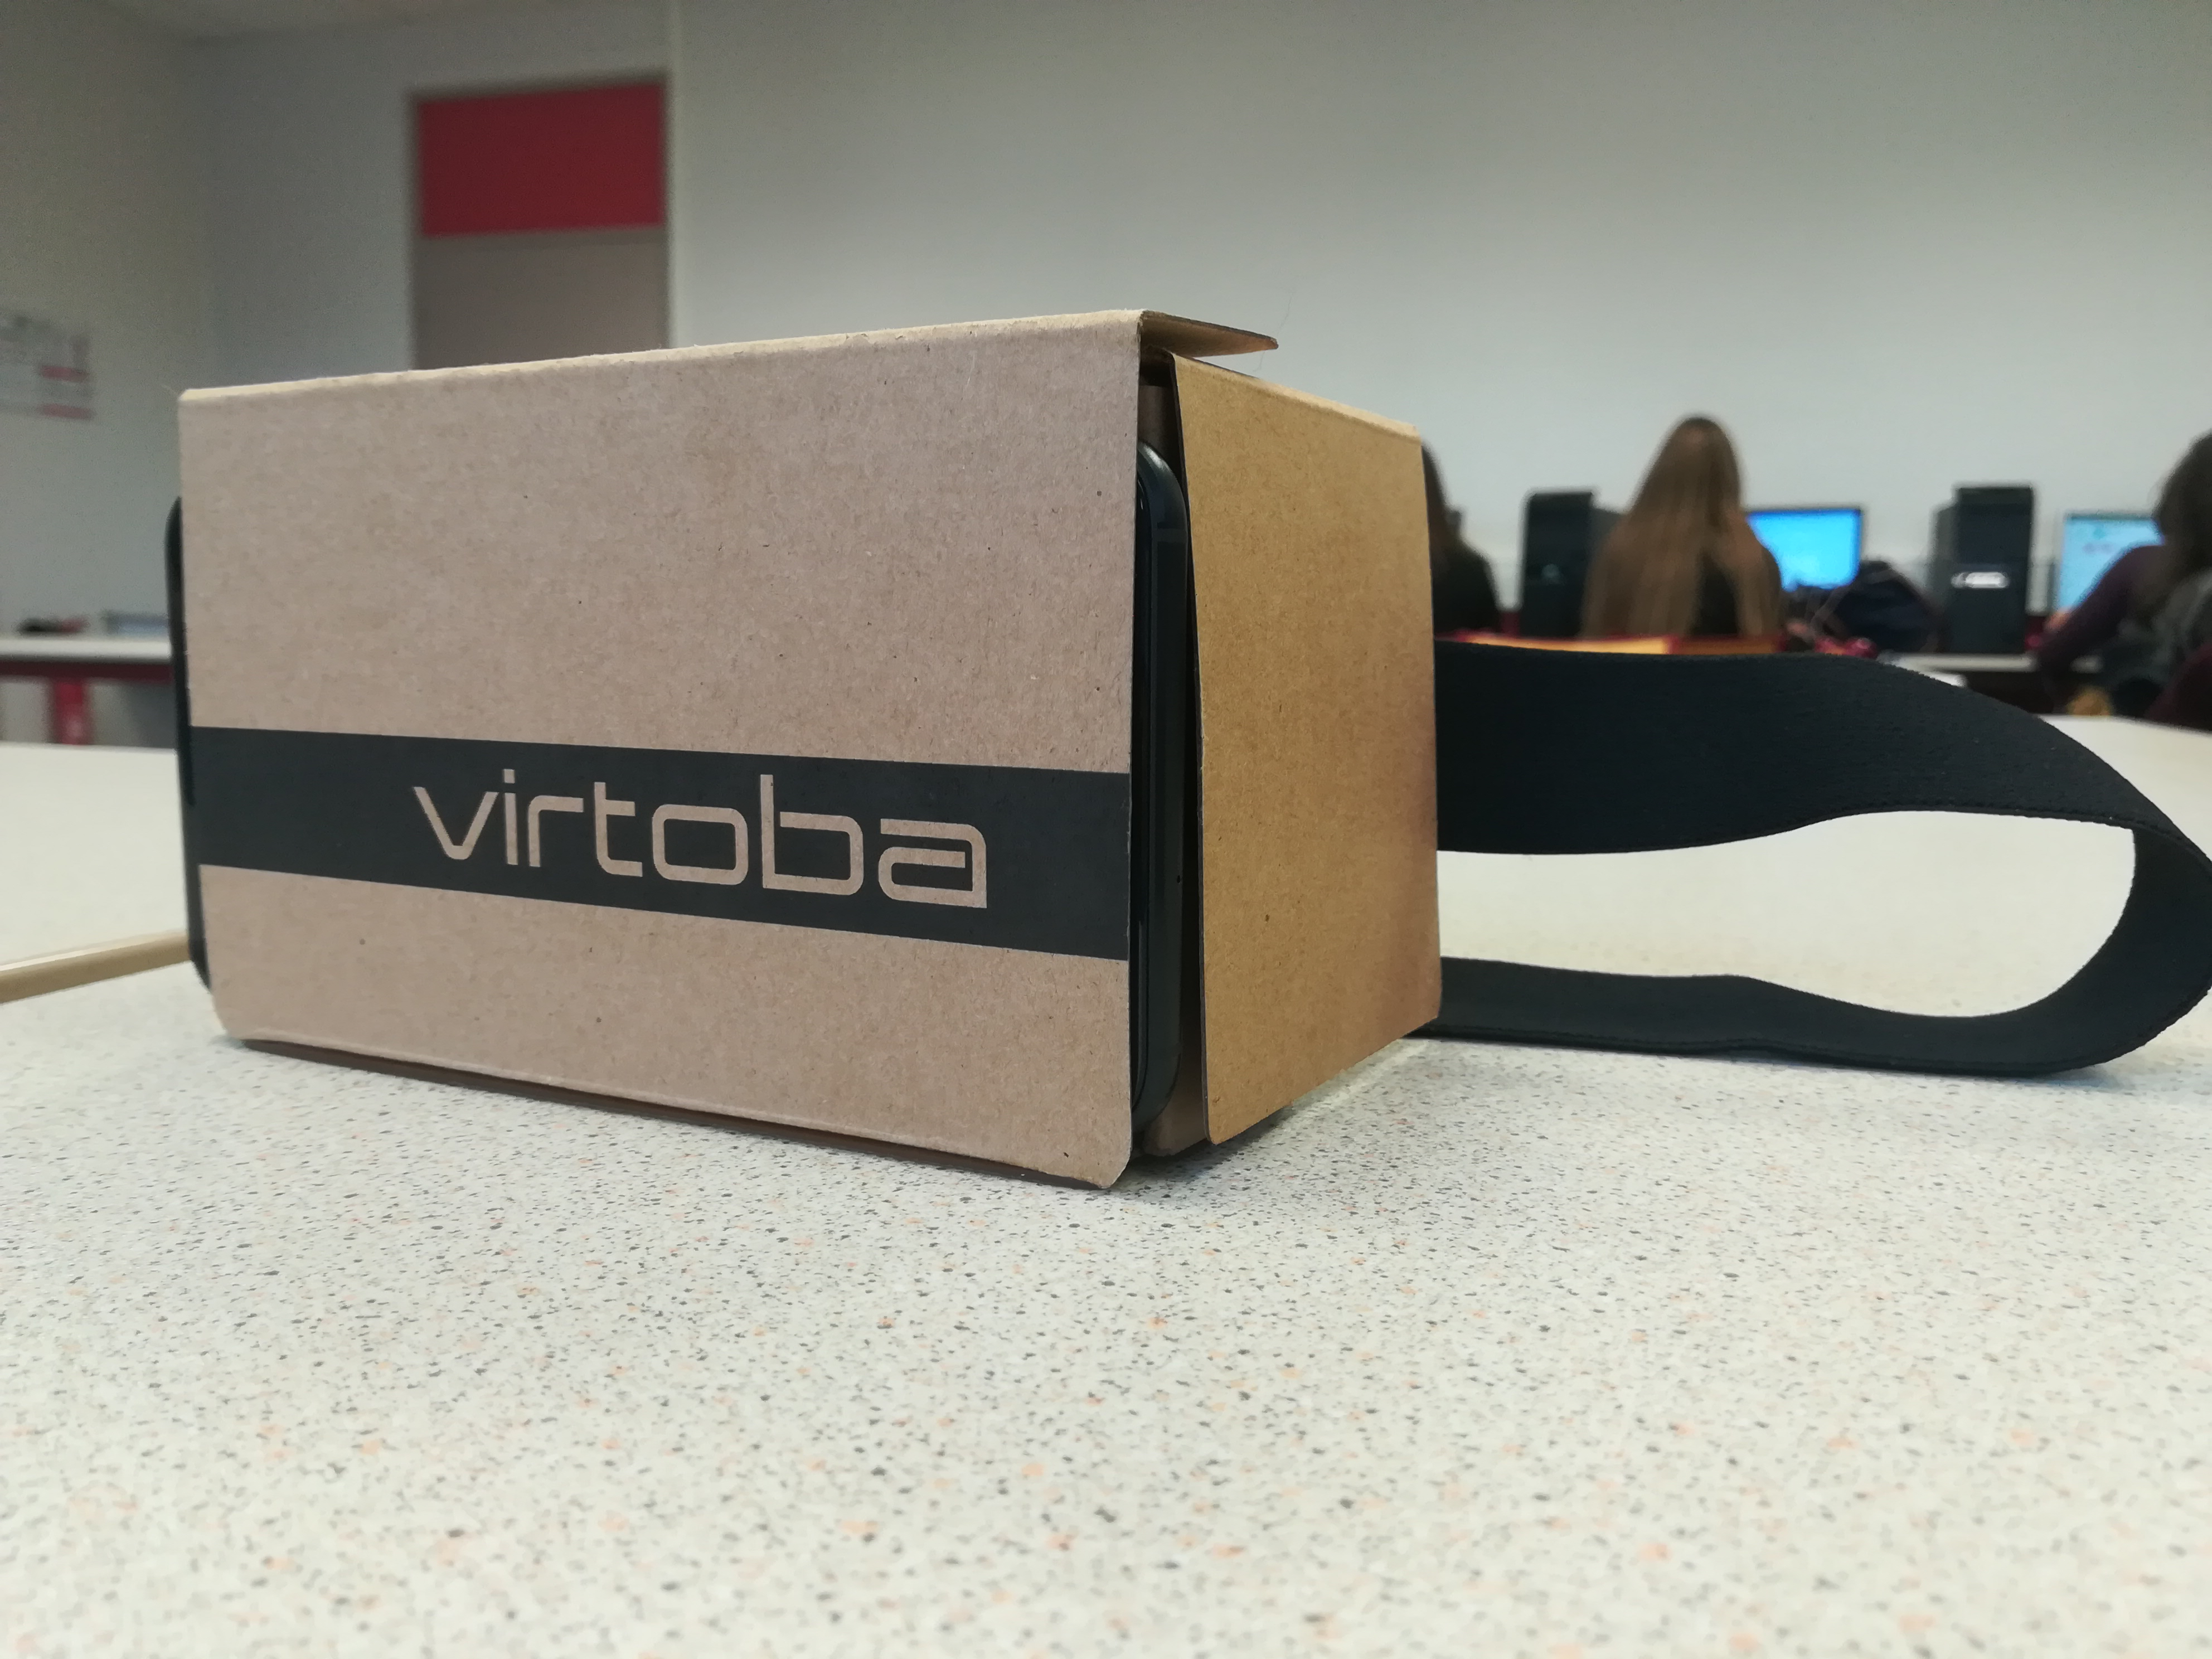
\includegraphics[scale=0.04]{carton.jpg}
\captionof{figure}{Le dispositif Google Cardboard}
\end{center}


\begin{center}
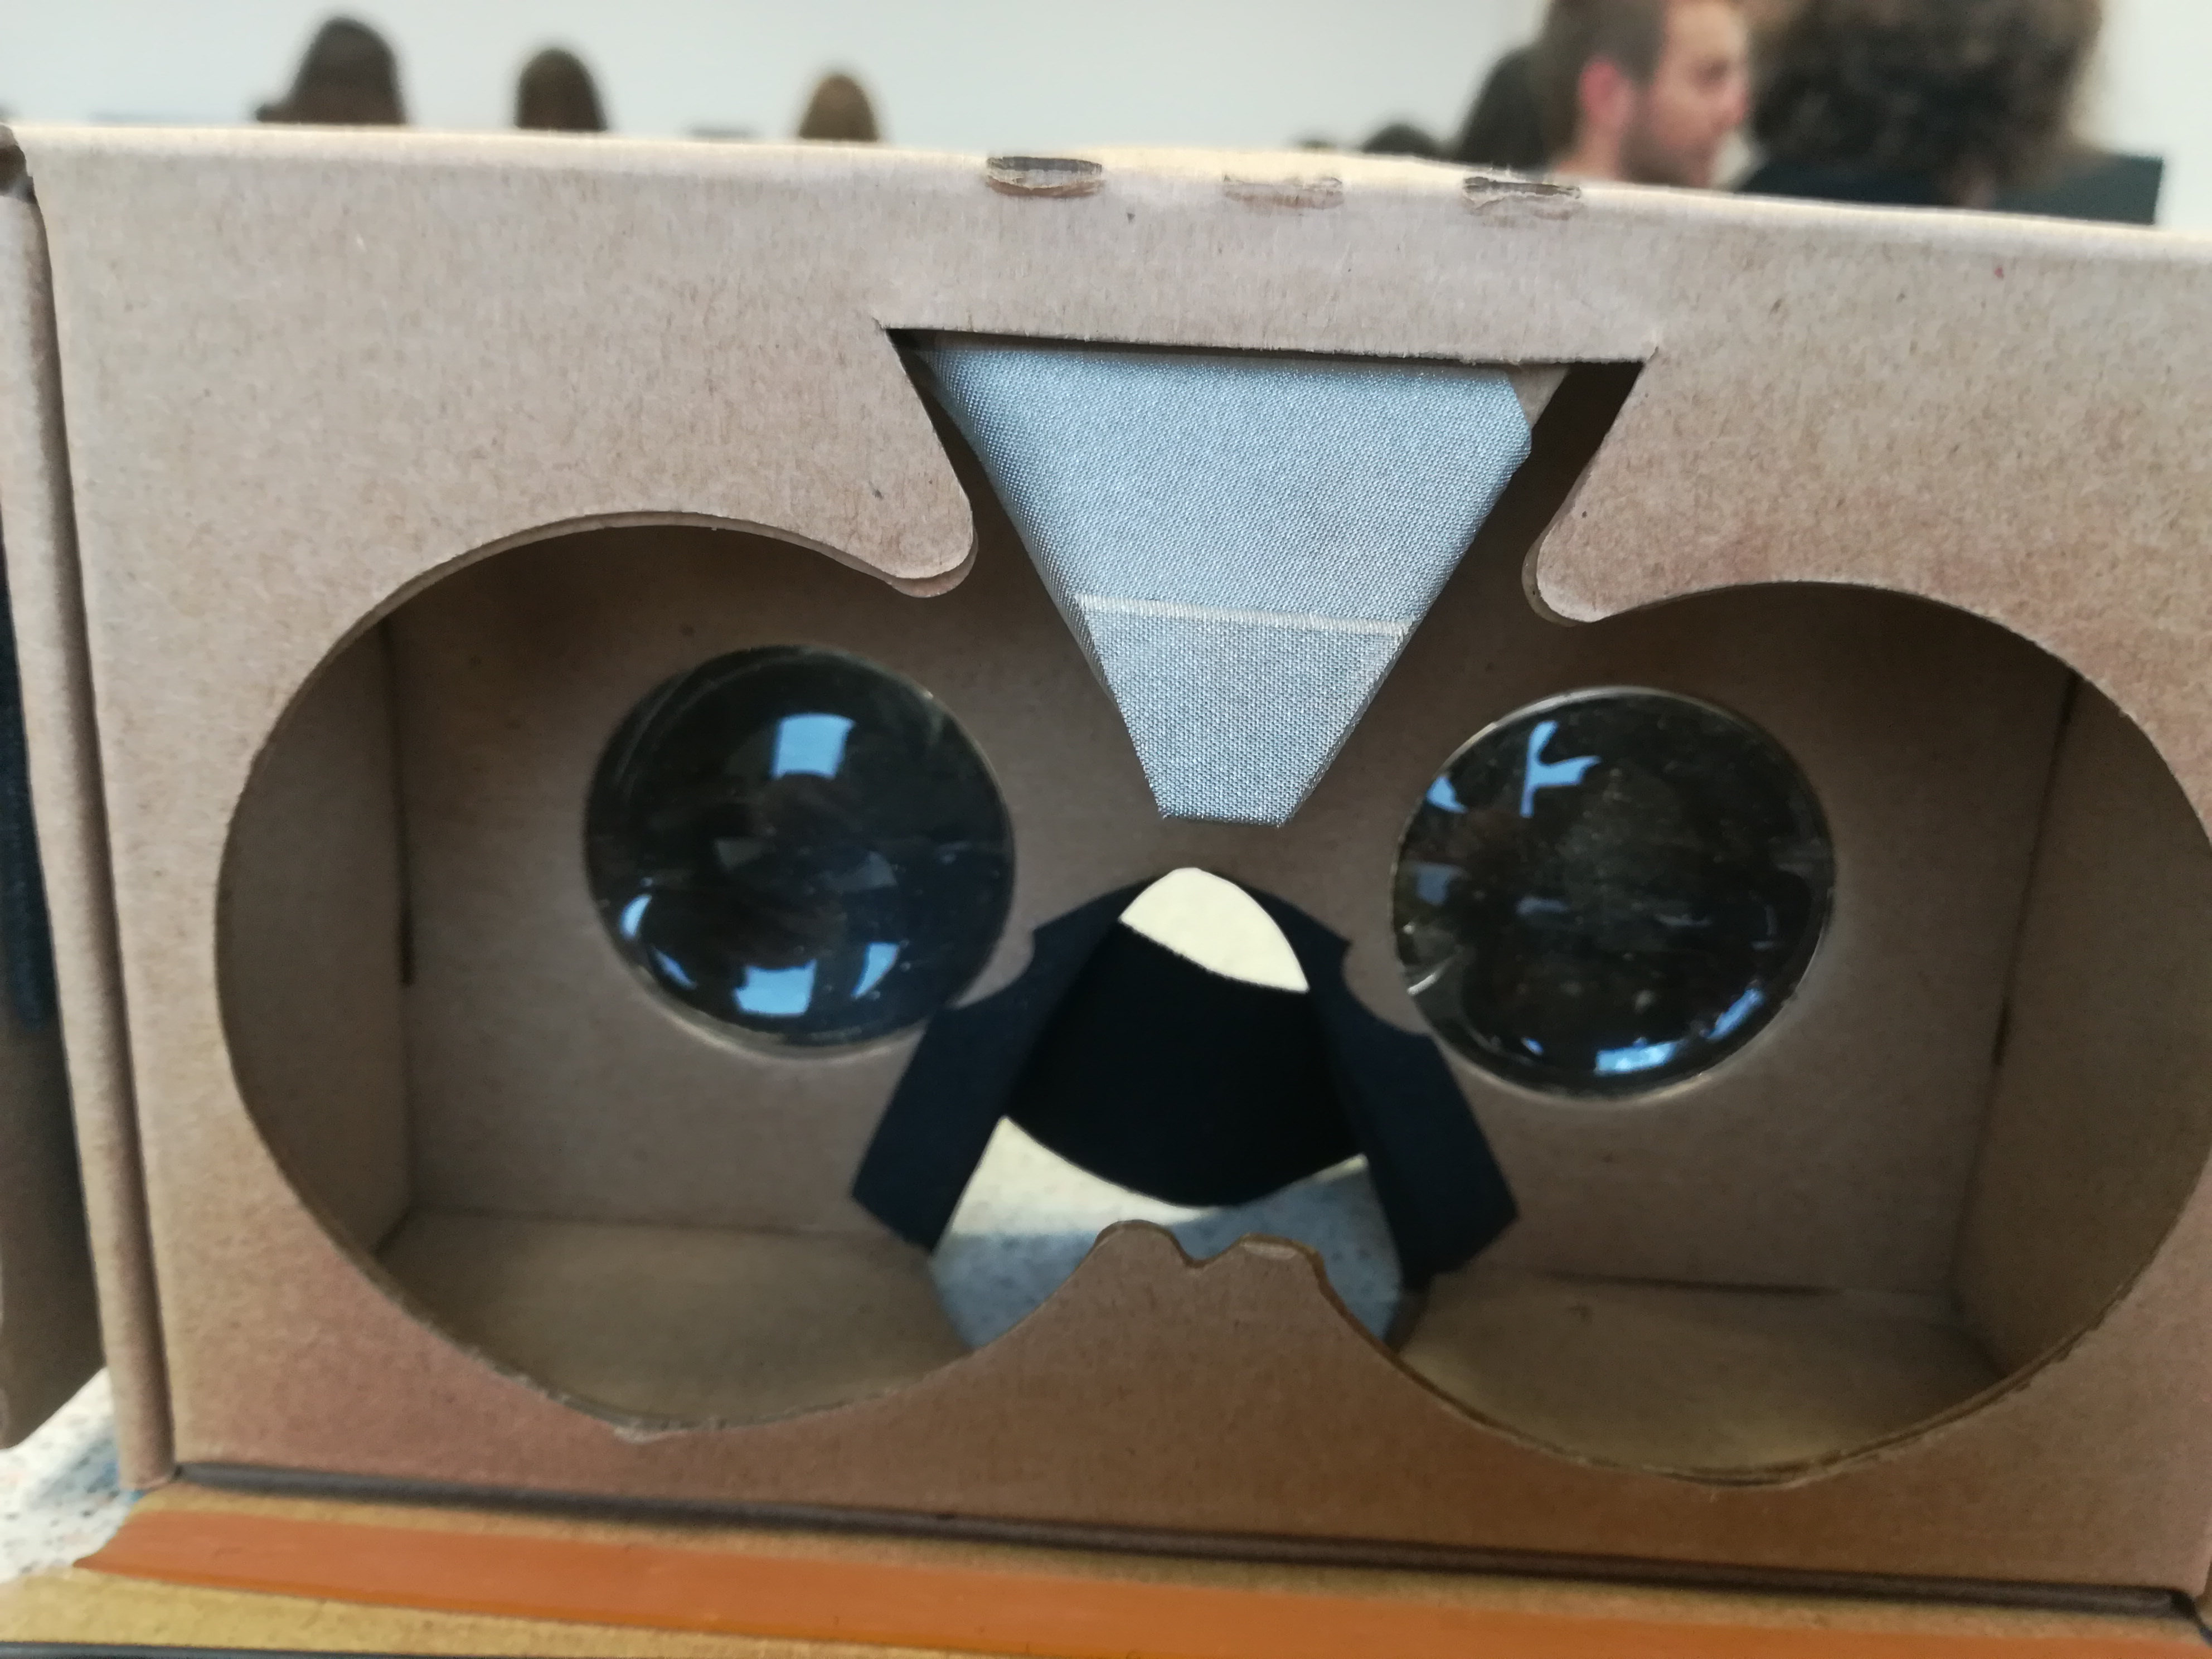
\includegraphics[scale=0.04]{card.jpg}
\captionof{figure}{L'intérieur du dispositif}
\end{center}

\begin{center}
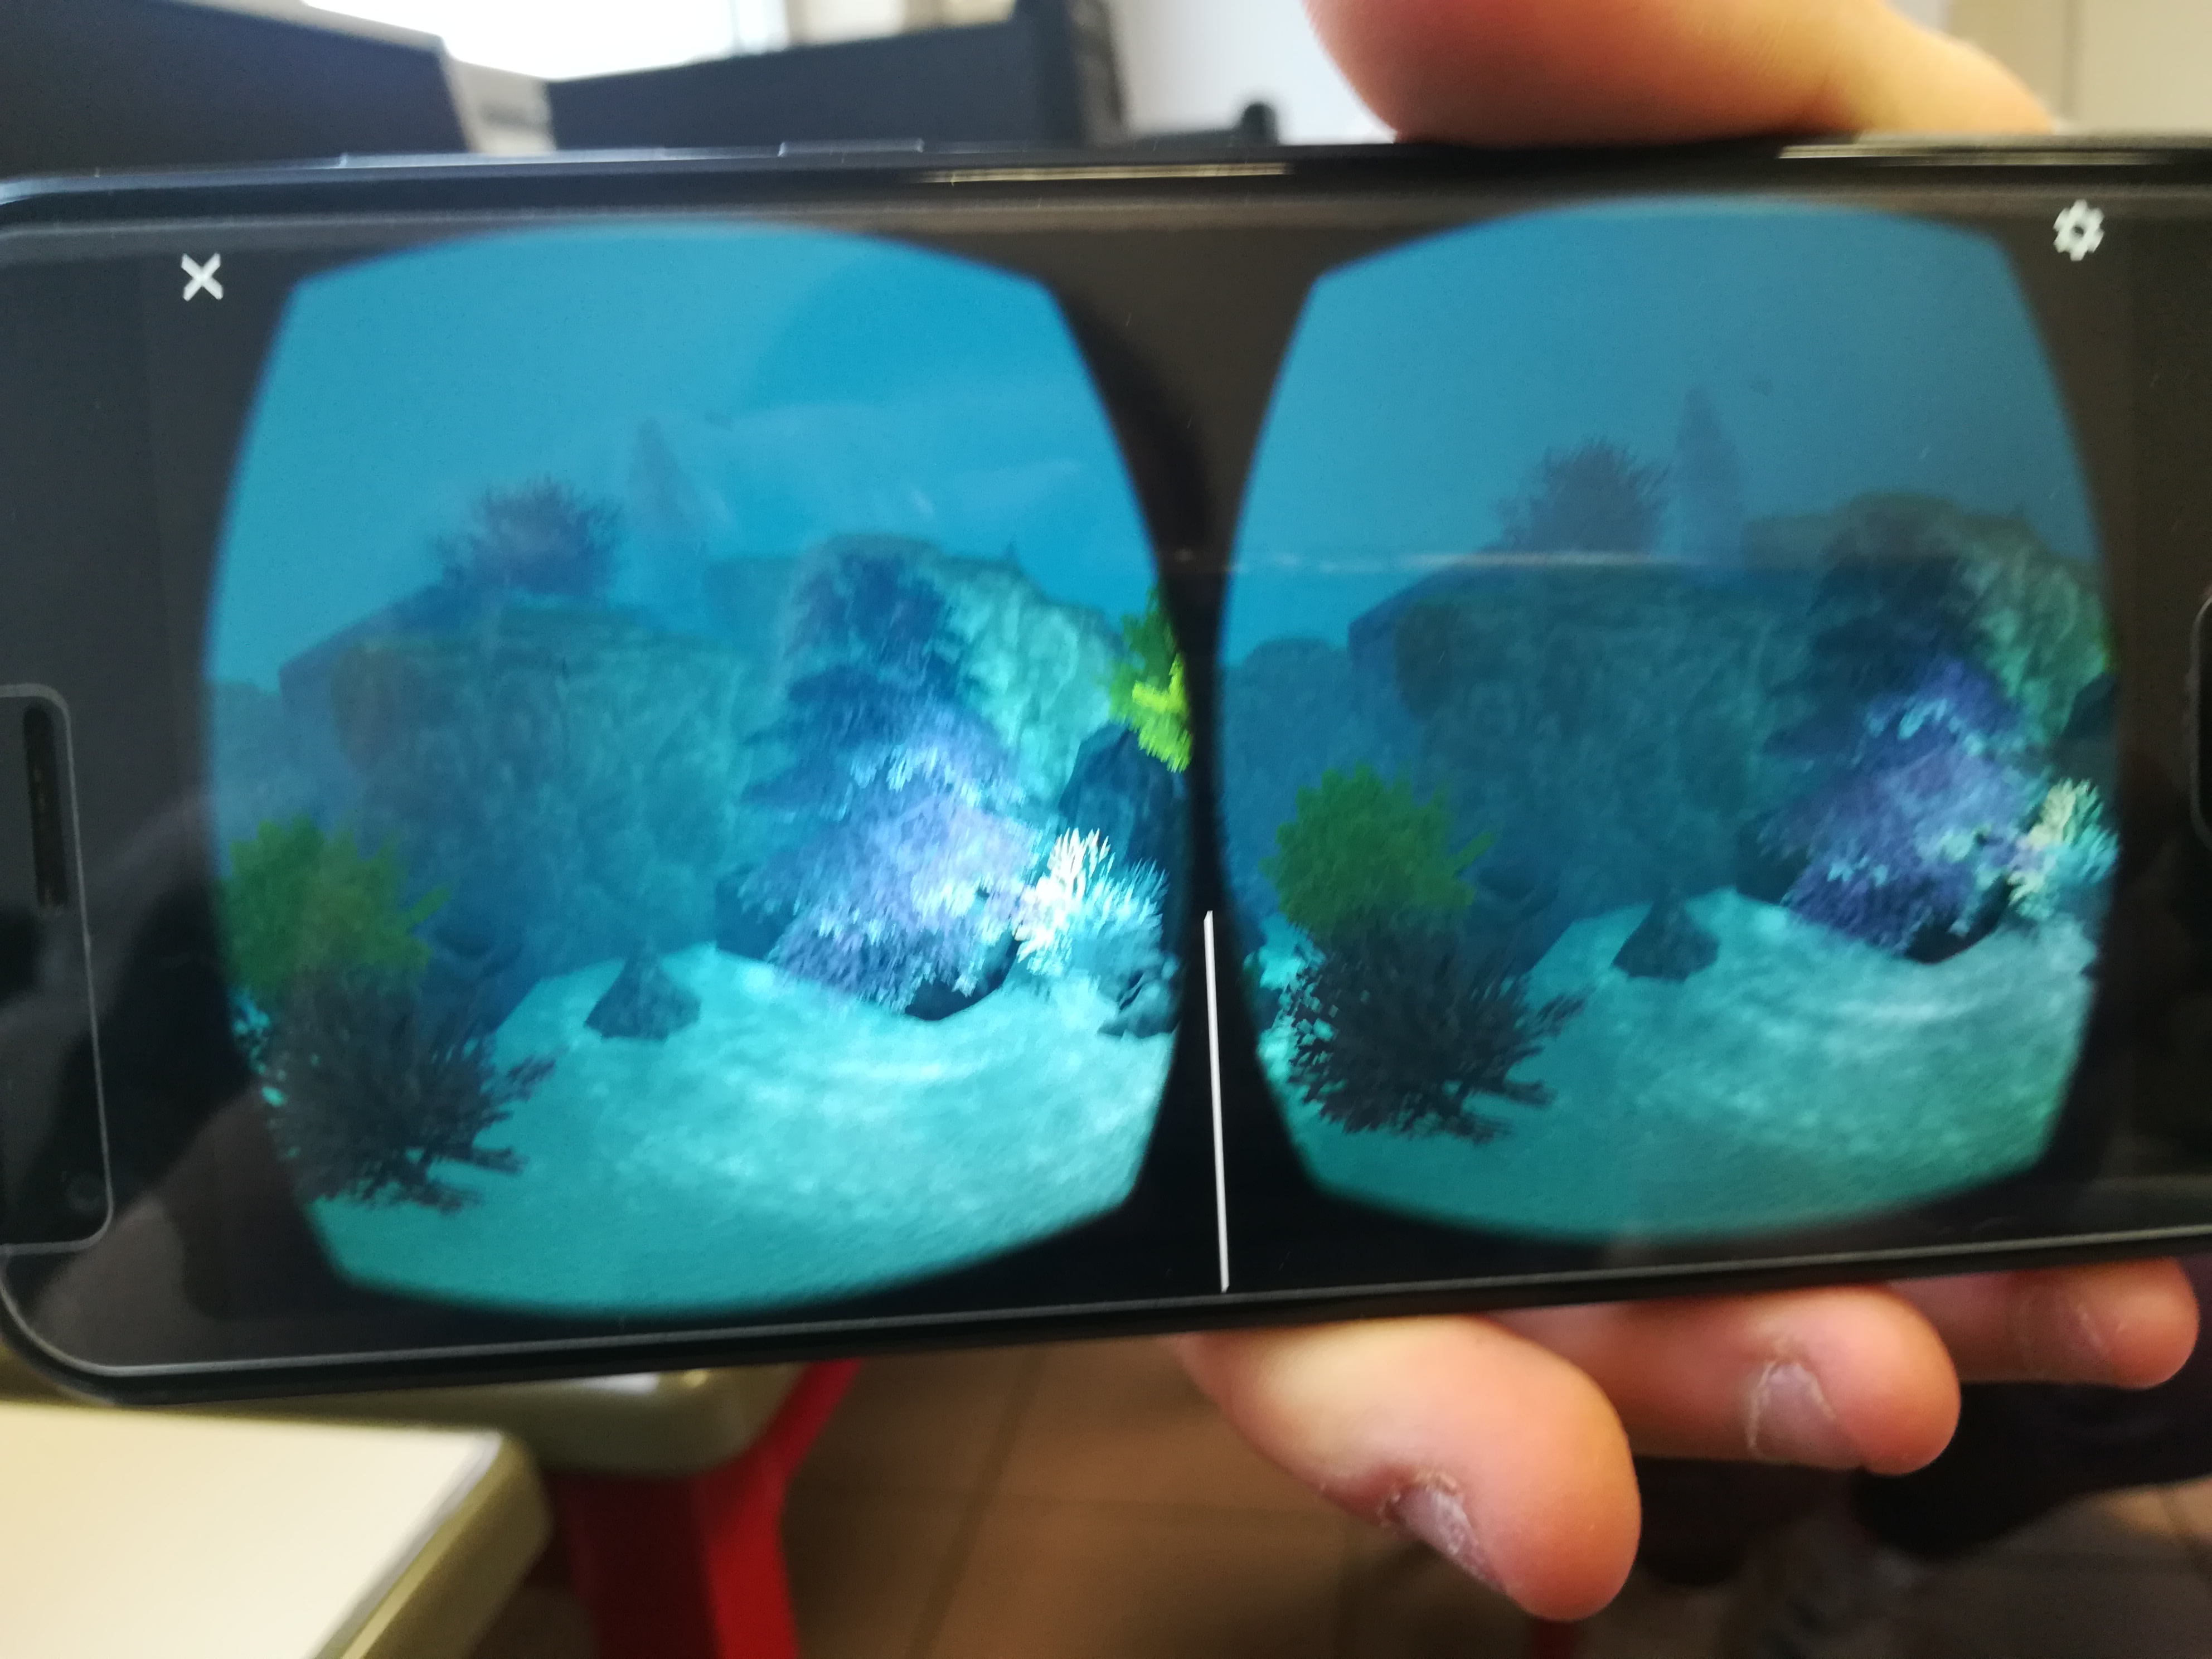
\includegraphics[scale=0.04]{telephone.jpg}
\captionof{figure}{Photographie de l'écran du téléphone}
\end{center}

Ainsi, les membres du jury pourront vivre une expérience de réalité virtuelle, tout comme nous avons pu en vivre une.

{\color{white}
\cite{1} \cite{2} \cite{3} \cite{4} \cite{5} \cite{6} \cite{7} \cite{8} \cite{9} \cite{10} \cite{11} \cite{12} \cite{13} \cite{14}
}

\addcontentsline{toc}{section}{Liste des figures}

\listoffigures{}

\addcontentsline{toc}{section}{Bibliographie}

\printbibliography{}

%%%%%%%%%%%%%%%%%%%%%%%%%%%%%%%%%%%%%%%%%%%%%%%%%%%%%%%%%%%%%%%%%%%%%%%%%%%%%%%

\end{document}